%
% File emnlp2018.tex
%
%% Based on the style files for EMNLP 2018, which were
%% Based on the style files for ACL 2018, which were
%% Based on the style files for ACL-2015, with some improvements
%%  taken from the NAACL-2016 style
%% Based on the style files for ACL-2014, which were, in turn,
%% based on ACL-2013, ACL-2012, ACL-2011, ACL-2010, ACL-IJCNLP-2009,
%% EACL-2009, IJCNLP-2008...
%% Based on the style files for EACL 2006 by 
%%e.agirre@ehu.es or Sergi.Balari@uab.es
%% and that of ACL 08 by Joakim Nivre and Noah Smith

\documentclass[11pt,a4paper]{article}
\usepackage[hyperref]{emnlp2018}
\usepackage{times}
\usepackage{latexsym}

\usepackage{url}

\aclfinalcopy % Uncomment this line for the final submission
\def\aclpaperid{1090} %  Enter the acl Paper ID here

%\setlength\titlebox{5cm}
% You can expand the titlebox if you need extra space
% to show all the authors. Please do not make the titlebox
% smaller than 5cm (the original size); we will check this
% in the camera-ready version and ask you to change it back.

% \renewcommand{\baselinestretch}{0.992}

\newcommand{\shaycomment}[1]{\textcolor{blue}{#1}}

\newcommand\BibTeX{B{\sc ib}\TeX}
\newcommand\confname{EMNLP 2018}
\newcommand\conforg{SIGDAT}

% Shashi
\usepackage{amsmath}
\usepackage{mathtools}
\mathtoolsset{showonlyrefs}
\usepackage{amssymb}
\usepackage{multirow}

\usepackage{tree-dvips}
\usepackage{pgf,tikz}
\usepackage{tikz-qtree}
\usepackage{graphicx}

\usepackage{lipsum}  
\definecolor{forestgreen}{HTML}{009B55}
\definecolor{sepia}{HTML}{671800}
\definecolor{midnightblue}{HTML}{006795}
\definecolor{orangered}{HTML}{ED135A}
\newcommand\refresh{\textsc{Refresh}}

\newcommand{\shashi}[1]{\textcolor{red}{TODO: #1}}

\title{Don't Give Me the Details, Just the Summary! \\Topic-Aware
  Convolutional Neural Networks for Extreme Summarization}

%\title{Topic-Aware Convolutional Sequence to Sequence Model for
 % Extreme Summarization}
% A Topic-Informed Model for Global Reasoning and Abstraction}
% Extreme Summarization: A Topic-Informed Model for Global Reasoning and Abstraction
% What is this Article about? A Topic-Informed Model for Extreme Summarization
% Topically Informed Model for Global Reasoning, Abstraction and Paraphrasing
% Topically Informed Model for Global Reasoning and Abstraction
% A Topic-Aware Model for Global Reasoning and Abstraction
% {Learning to Reason and Abstract: An Extreme Case of Document Summarization} 
% Topically Informed Model for Global Inference and Abstraction
% {Extreme Document Summarization} % Automatic Generation of Story Introduction}

% \author{First Author \\
%   Affiliation / Address line 1 \\
%   Affiliation / Address line 2 \\
%   Affiliation / Address line 3 \\
%   {\tt email@domain} \\\And
%   Second Author \\
%   Affiliation / Address line 1 \\
%   Affiliation / Address line 2 \\
%   Affiliation / Address line 3 \\
%   {\tt email@domain} \\}

\author{Shashi Narayan \quad Shay B. Cohen \quad Mirella Lapata \\ 
  Institute for Language, Cognition and Computation \\
  School of Informatics, University of Edinburgh \\ 
  10 Crichton Street, Edinburgh, EH8 9AB  \\ 
  \texttt{\url{shashi.narayan@ed.ac.uk}},
  \texttt{\{scohen,mlap\}@inf.ed.ac.uk} 
}

\makeatletter
\newcommand{\thickhline}{%
    \noalign {\ifnum 0=`}\fi \hrule height 1pt
    \futurelet \reserved@a \@xhline
}
\makeatother

\date{}

\begin{document}
\maketitle
\begin{abstract}

  We introduce \emph{extreme summarization}, a new single-document
  summarization task which does not favor extractive strategies and
  calls for an abstractive modeling approach. The idea is to create a
  short, one-sentence news summary answering the question ``What is
  the article about?''. We collect a real-world, large scale dataset
  for this task by harvesting online articles from the British
  Broadcasting Corporation (BBC). We propose a novel abstractive model
  which is conditioned on the article's topics and based entirely on
  convolutional neural networks.  We demonstrate experimentally that
  this architecture captures long-range dependencies in a document and
  recognizes pertinent content, outperforming an oracle extractive
  system and state-of-the-art abstractive approaches when evaluated
  automatically and by humans.\footnote{Our dataset, code, and demo
    are available at: \url{https://github.com/shashiongithub/XSum}.}

%  This abstractive model is better in modeling long-range
%  dependencies in the document and recognizing pertinent content. We
%  demonstrate experimentally that our model outperforms an oracle
%  extractive system and state-of-the-art abstractive systems when
%  evaluated automatically and by humans.
\end{abstract}

% Introduction
\section{Introduction}

Automatic summarization is one of the central problems in Natural
Language Processing (NLP) posing several challenges relating to {\em
  understanding} (i.e.,~identifying important content) and {\em
  generation} (i.e.,~aggregating and rewording the identified
content into a summary). Of the many summarization paradigms that have
been identified over the years (see \citeauthor{mani2001automatic},
\citeyear{mani2001automatic} and \citeauthor{Nenkova:McKeown:2011},
\citeyear{Nenkova:McKeown:2011} for a comprehensive overview),
single-document summarization has consistently attracted attention
\cite{jp-acl16,durrett-nyt-ext,nallapati-signll16,nallapati17,see-acl17,tanwan-acl17,narayan-arxiv17,Fan2017Controllable,paulus-socher-arxiv17,Pasunuru-multireward18,asli-multiagent18,narayan-sidenet18,narayan-rank18}.


\begin{figure}[t!]
  \center{\fontsize{10}{12}\selectfont % \footnotesize % \small % scriptsize % footnotesize
    \begin{tabular}{ p{7.2cm} }
      \thickhline
      
     % \vspace{0.01cm}
      
      \textbf{\textsc{Summary:}} \emph{\textcolor{orangered}{A man and
          a child have been killed} after a \textcolor{sepia}{light}
        \textcolor{forestgreen}{aircraft made an emergency landing} on
        \textcolor{midnightblue}{a beach in Portugal}.}  
       \\ \thickhline
      
      \textbf{\textsc{Document:}} Authorities said the incident took place on \textcolor{midnightblue}{Sao Joao beach in Caparica, south-west of Lisbon}. \\ 

      The National Maritime Authority said \textcolor{orangered}{a middle-aged man and a young girl died} after they were unable to avoid the plane. \\
      
      [{\em 6 sentences with 139 words are abbreviated from here.}] \\
      
      % The plane's only two occupants were unharmed, it added. \\

      % The Diario de Noticias newspaper quoted an eyewitness who said the plane had been flying at a low altitude over the beach, although he did not realise anything was wrong until other beachgoers began running. \\

      % One young witness told Reuters news agency: "I was near the water when I saw the plane. I called my parents, the plane fell on the sand and ran over two people, fatally hurting them and another was injured, I think, but I'm not sure, people were running away. \\

      % "The plane is still there, but the ambulances arrived quickly. I think maybe the fuel ran out because I find it weird that it landed on the beach." \\

      Other reports said the victims had been sunbathing when \textcolor{forestgreen}{the plane made its emergency landing}. \\

      [{\em Another 4 sentences with 67 words are abbreviated from here.}] \\

      % The Associated Press news agency said the girl who died had been with her parents, who were unhurt. The agency quoted witnesses from local television broadcasts. \\

      % Joao Quadros, who was on the beach, tweeted photos of the aftermath, saying the plane had passed by his son by a matter of metres. There had been no noise, he said. \\ 

      Video footage from the scene carried by local broadcasters showed \textcolor{sepia}{a small recreational plane} parked on the sand, apparently intact and surrounded by beachgoers and emergency workers. % One wing seemed to be misaligned in those photos.
      \\

      % The cause of the emergency landing remains unclear.
      % \\
        
      [{\em Last 2 sentences with 19 words are abbreviated.}] \\
      
      \thickhline
    \end{tabular}     
  }
  \caption{An abridged example from our extreme summarization dataset
    showing the document and its one-line summary. Document content
    present in the summary is color-coded.
    %The summary exemplifies across-the-document reasoning to identify important content and 
    %multiple levels of abstraction such as sentence fusion % ,
                                                           % synthesis
    %and paraphrasing. 
    % Title: Two killed in Portugal beach plane crash
    % url: http://www.bbc.co.uk/news/world-europe-40806376
  }\label{fig:bbcex-1}
\end{figure}

Neural approaches to NLP and their ability to learn continuous
features without recourse to pre-processing tools or linguistic
annotations have driven the development of large-scale document
summarization datasets
\cite{nytcorpus,hermann-nips15,newsroom-naacl18}.
% and their \shaycomment{ability of what? approach? neural networks? grammatically confusing}
% ability to learn continuous features
% without recourse to preprocessing tools or linguistic annotations has
% driven the development and use of large scale single document
% summarization datasets
% \cite{nytcorpus,hermann-nips15,newsroom-naacl18}.
However, these datasets often favor extractive models which create a
summary by identifying (and subsequently concatenating) the most
important sentences in a document
\cite{jp-acl16,nallapati17,narayan-rank18}.  Abstractive approaches,
despite being more faithful to the actual summarization task, either
lag behind extractive ones or are mostly extractive, exhibiting a
small degree of abstraction
\cite{see-acl17,tanwan-acl17,paulus-socher-arxiv17,Pasunuru-multireward18,asli-multiagent18}.


In this paper we introduce \emph{extreme summarization}, a new
single-document summarization task which is not amenable to extractive
strategies and requires an abstractive modeling approach. The idea is
to create a short, one-sentence news summary answering the question
``What is the article about?''. An example of a document and its
extreme summary are shown in Figure~\ref{fig:bbcex-1}. As can be seen,
the summary is very different from a headline whose aim is to
encourage readers to read the story; it draws on information
interspersed in various parts of the document (not only the beginning)
and displays multiple levels of abstraction including paraphrasing,
fusion, synthesis, and inference. We build a dataset for the proposed
task by harvesting online articles from the British Broadcasting
Corporation (BBC) that often include a first-sentence summary.
%answering ``What is the article about?''  Extreme summarization aims
%at generating the first sentence from the rest of the article.





%address the issue of this ``extractive bias''.  We
%introduce a new single document summarization task, ``extreme
%summarization,'' which does not favor extractive strategies and
%essentially requires abstractive summarization. 

%Figure~\ref{fig:bbcex-1} shows an example article
%from our dataset. Information to assemble the summary comes from
%different depths of the document demanding multiple levels of
%abstractions including paraphrasing, fusion, synthesis and
%inference. By the virtue of this task, it presents more challenges
%than extractive summarization while upholding the important
%characteristics of NLP and document summarization.


We further propose a novel deep learning model which we argue is
well-suited to the extreme summarization task. Unlike most existing
abstractive approaches
\cite{rush-acl15,chenIjcai-16,nallapati-signll16,see-acl17,tanwan-acl17,paulus-socher-arxiv17,Pasunuru-multireward18,asli-multiagent18}
which rely on an encoder-decoder architecture modeled by recurrent
neural networks (RNNs), we present a \emph{topic-conditioned} neural
model which is based entirely on convolutional neural networks
\cite{convseq2seq}. Convolution layers capture long-range
dependencies between words in the document more effectively compared to
RNNs, allowing to perform document-level inference, abstraction, and
paraphrasing.  Our convolutional encoder associates each word with a
topic vector capturing whether it is representative of the document's
content, while our convolutional decoder conditions each word
prediction on a document topic vector.


%and that are prone to mishandling long-range
%dependencies, we present a topic-conditioned convolutional
%sequence-to-sequence which allows document-level inference,
%abstraction and paraphrasing.  
%
%Our models adapts an architecture based
%entirely on convolutional neural networks (\textsc{ConvS2S},
%\citeauthor{convseq2seq}, \citeyear{convseq2seq}). We stack
%convolution layers to model long-range dependencies between words in
%the document effectively; they provide a shorter path to capture
%relationship between distant words in the document compared to RNNs.



% words at closer distances interact at lower layers while distant
% words interact at higher layers.
%In addition, we improve the convolutional
%encoder by associating each word with a topic vector capturing ``how
%topical is a word in the document?'' and the convolutional decoder by
%conditioning each word prediction on the document topic vector.


Experimental results show that when evaluated automatically (in terms
of ROUGE) our topic-aware convolutional model outperforms an oracle
extractive system and state-of-the-art RNN-based abstractive
systems. We also conduct two human evaluations in order to assess (a)
which type of summary participants prefer and (b) how much key
information from the document is preserved in the summary. Both
evaluations overwhelmingly show that human subjects find our summaries
more informative and complete. Our contributions in this work are
three-fold: a new single document summarization dataset that
encourages the development of abstractive systems; corroborated by
analysis and empirical results showing that extractive approaches are
not well-suited to the extreme summarization task; and a novel
topic-aware convolutional sequence-to-sequence model for abstractive
summarization.
%and an additional novel topic-conditioned model for summarization
%(also based on convolutional seq2seq modeling).


%%% Local Variables:
%%% mode: latex
%%% TeX-master: "extreme-sum"
%%% End:



% XSum Dataset

\section{The XSum Dataset}
\label{sec:bbcdataset}

% \begin{table*}[ht]
%   \begin{center}{\footnotesize
%   \begin{tabular}{ l | l | c c | c c | r r}
%     \thickhline
%     \multirow{2}{*}{Datasets} & \multirow{2}{*}{\# docs (train/val/test)} & \multicolumn{2}{c|}{avg. document length} & \multicolumn{2}{c|}{avg. summary length} & \multicolumn{2}{c}{vocabulary size}\\
%     & & words & sentences & words & sentences & document & summary\\ \thickhline 
%     CNN & 90,266/1,220/1,093 & 760.50 & 33.98 & 45.70 & 3.59 & 343,516 & 89,051 \\
%     DailyMail & 196,961/12,148/10,397 & 653.33 & 29.33 & 54.65 & 3.86 & 563,663 & 179,966 \\
%     NY Times & 589,284/32,736/32,739 & 800.04 & 35.55 & 45.54 & 2.44 & 1,399,358 & 294,011 \\ 
%     Newsroom & 992,966/108,591/108,650 & 770.09 & 34.73 & 30.36 & 1.43 & 2,646,681 & 360,290\\ \hline
%     Newsroom-ext & 331,778/36,332/36,122 & 706.06 & 31.65 & 45.78 & 1.88 & 1,214,748 & 243,062 \\
%     Newsroom-mixed & 328,634/35,879/36,006 & 830.58 & 36.63 & 23.78 & 1.17 & 1,271,435 & 169,875 \\
%     Newsroom-abs & 332,554/36,380/36,522 & 774.17 & 35.92 & 21.49 & 1.25 & 1,385,205 & 157,939 \\ \hline
%     XSum & 204,045/11,332/11,334 & 431.07 & 19.77 & 23.26 & 1.00 & 399,147 & 81,092 \\ \thickhline
%   \end{tabular}}
%   \end{center}
%   \caption{We compare  datasets
%     with respect to overall corpus size, size of training, validation,
%     and test sets, average document (source) and summary (target)
%     length (in terms of words and sentences), and  vocabulary size on
%     both on source and target. For CNN and DailyMail,
%     we  used the original splits of
%     \protect\newcite{hermann-nips15} and followed
%     \protect\newcite{narayan-rank18} to preprocess them. For  NY
%     Times  \protect\cite{nytcorpus}, we  used the splits
%     and pre-processing steps of
%     \protect\newcite{paulus-socher-arxiv17}. For the Newsroom dataset, we use the splits
%     and pre-processing steps of \protect\newcite{newsroom-naacl18}. We present the full 
%     Newsroom dataset (Newsroom) along with its three subsets: mostly extractive (Newsroom-ext), 
%     mixed (Newsroom-mixed) and mostly abstractive (Newsroom-abs).
%     For the vocabulary, we
%     lower case tokens. } \label{table:bbc-size-comparison} 
% \end{table*}

\begin{table*}
  \begin{center}{\footnotesize
  \begin{tabular}{ l | l | c c | c c | r r}
    \thickhline
    \multirow{2}{*}{Datasets} & \multirow{2}{*}{\# docs (train/val/test)} & \multicolumn{2}{c|}{avg. document length} & \multicolumn{2}{c|}{avg. summary length} & \multicolumn{2}{c}{vocabulary size}\\
    & & words & sentences & words & sentences & document & summary\\ \thickhline 
    CNN & 90,266/1,220/1,093 & 760.50 & 33.98 & 45.70 & 3.59 & 343,516 & 89,051 \\
    DailyMail & 196,961/12,148/10,397 & 653.33 & 29.33 & 54.65 & 3.86 & 563,663 & 179,966 \\
    NY Times & 589,284/32,736/32,739 & 800.04 & 35.55 & 45.54 & 2.44 & 1,399,358 & 294,011 \\
    XSum & 204,045/11,332/11,334 & 431.07 & 19.77 & 23.26 & 1.00 & 399,147 & 81,092 \\ \thickhline
  \end{tabular}}
  \end{center}
  \caption{Comparison of summarization datasets
    with respect to overall corpus size, size of training, validation,
    and test set, average document (source) and summary (target)
    length (in terms of words and sentences), and  vocabulary size on
    both on source and target. For CNN and DailyMail,
    we  used the original splits of
    \protect\newcite{hermann-nips15} and followed
    \protect\newcite{narayan-rank18} to preprocess them. For  NY
    Times  \protect\cite{nytcorpus}, we  used the splits
    and pre-processing steps of
    \protect\newcite{paulus-socher-arxiv17}. For the vocabulary, we
    lowercase tokens.} \label{table:bbc-size-comparison} 
\end{table*}

% \begin{table*}
%   \begin{center}{\footnotesize
%   \begin{tabular}{ l | c c c c | c c c | c c c } %  l l l l | l l l | l l l}
%     \thickhline
%     \multirow{2}{*}{Datasets} & \multicolumn{4}{c|}{\% of novel n-grams in gold summary} & \multicolumn{3}{c|}{\textsc{lead}} & \multicolumn{3}{c}{\textsc{ext-oracle}} \\
%     & unigrams & bigrams & trigrams & 4-grams & R1 & R2 & RL & R1 & R2 & RL \\ \thickhline 
%     CNN & 16.75 & 54.33 & 72.42 & 80.37 & 29.15 & 11.13 & 25.95 & 50.38 & 28.55 & 46.58 \\
%     DailyMail & 17.03 & 53.78 & 72.14 & 80.28 & 40.68 & 18.36 & 37.25 & 55.12 & 30.55 & 51.24 \\
%     NY Times & 22.64 & 55.59 & 71.93 & 80.16 & 31.85 & 15.86 & 23.75 & 52.08 & 31.59 & 46.72 \\ 
%     Newsroom & 18.31 & 46.80 & 58.06 & 62.72 & 33.04 & 22.35 & 30.31 & 57.09 & 42.94 & 53.65 \\ \hline
%     Newsroom-ext & 2.65 & 7.25 & 10.25 & 12.42 & 55.87 & 50.60 & 54.76 & 89.63 & 87.20 & 89.32 \\
%     Newsroom-mixed & 13.78 & 48.37 & 67.15 & 77.11 & 27.95 & 13.87 & 23.97 & 51.98 & 34.04 & 46.96 \\ 
%     Newsroom-abs & \textbf{38.25} & \textbf{84.36} & \textbf{96.39} & 98.28 & \textbf{15.44} & 2.72 & 12.32 & 29.85 & \textbf{7.82} & 24.86\\ \hline
%     XSum & 35.76 & 83.45  & 95.50  & \textbf{98.49}  & 16.30 & \textbf{1.61}  & \textbf{11.95}  & \textbf{29.79}  & 8.81  & \textbf{22.65}  \\ \thickhline
%   \end{tabular}}
%   \end{center}
%   \caption{Corpus bias towards extractive methods in the CNN,
%     DailyMail, NY Times, Newsroom, and XSum datasets.  We show  the proportion of novel $n$-grams in gold summaries. We also report ROUGE scores  for
%     the  \textsc{lead} baseline and 
%     \textsc{ext-oracle}, the extractive oracle system.     All results
%     are computed on the test set.} \label{table:ngram-coverage-lead-oracle}
% \end{table*}

\begin{table*}
  \begin{center}{\footnotesize
  \begin{tabular}{ l | c c c c | c c c | c c c } %  l l l l | l l l | l l l}
    \thickhline
    \multirow{2}{*}{Datasets} & \multicolumn{4}{c|}{\% of novel n-grams in gold summary} & \multicolumn{3}{c|}{\textsc{lead}} & \multicolumn{3}{c}{\textsc{ext-oracle}} \\
    & unigrams & bigrams & trigrams & 4-grams & R1 & R2 & RL & R1 & R2 & RL \\ \thickhline 
    CNN & 16.75 & 54.33 & 72.42 & 80.37 & 29.15 & 11.13 & 25.95 & 50.38 & 28.55 & 46.58 \\
    DailyMail & 17.03 & 53.78 & 72.14 & 80.28 & 40.68 & 18.36 & 37.25 & 55.12 & 30.55 & 51.24 \\
    NY Times & 22.64 & 55.59 & 71.93 & 80.16 & 31.85 & 15.86 & 23.75 & 52.08 & 31.59 & 46.72 \\
    XSum & \textbf{35.76} & \textbf{83.45}  & \textbf{95.50}  & \textbf{98.49}  & \textbf{16.30} & \textbf{1.61}  & \textbf{11.95}  & \textbf{29.79}  & \textbf{8.81}  & \textbf{22.65}  \\ \thickhline
  \end{tabular}}
  \end{center}
  \caption{Corpus bias towards extractive methods in the CNN,
    DailyMail, NY Times, and XSum datasets.  We show  the proportion of novel $n$-grams in gold summaries. We also report ROUGE scores  for
    the  \textsc{lead} baseline and the extractive oracle system
    \textsc{ext-oracle}.     Results
    are computed on the test set.
    \label{table:ngram-coverage-lead-oracle}}
\end{table*}


%BBC articles often have
%their first sentence, tagged with an HTML class
%``story-body\_\_introduction,'' written to introduce the article.
%Our aim is to predict that sentence from the rest of the
%article.
%The first sentence in the BBC articles include important information from across the
%whole document, and as such generating it requires inference across the document.
%In addition, since we have one sentence at hand, generating it requires
%complex fusion, synthesis and paraphrasing. Figure \ref{fig:bbcex-1}
%shows an example article from our dataset exhibiting these operations.


Our extreme summarization dataset (which we call XSum) consists of BBC
articles and accompanying single sentence summaries. Specifically,
each article is prefaced with an introductory sentence (aka summary)
which is professionally written, typically by the author of the
article. The summary bears the HTML class
``story-body\_\_introduction,'' and can be easily identified and
extracted from the main text body (see Figure~\ref{fig:bbcex-1} for an
example summary-article pair).



% Discuss the example to promote the task. 

%\paragraph{Data Collection and Statistics.} 


We followed the methodology proposed in \newcite{hermann-nips15} to
create a large-scale dataset for extreme summarization. Specifically,
we collected~226,711 Wayback archived BBC articles ranging over almost
a decade (2010 to 2017) and covering a wide variety of domains
(e.g.,~News, Politics, Sports, Weather, Business, Technology, Science,
Health, Family, Education, Entertainment and Arts). Each article comes
with a unique identifier in its URL, which we used to randomly split
the dataset into training (90\%, 204,045), validation (5\%, 11,332),
and test (5\%, 11,334) set. Table~\ref{table:bbc-size-comparison}
compares XSum with the CNN, DailyMail, and NY Times % , and Newsroom
benchmarks. As can be seen, XSum contains a substantial number of
training instances, similar to DailyMail; documents and summaries in
XSum are shorter in relation to other datasets but the vocabulary size
is sufficiently large, comparable to CNN.

% grep 'web/2017' map-webarxive-bbcid.txt | wc -l 119262
% grep 'web/2016' map-webarxive-bbcid.txt | wc -l 70457
% grep 'web/2015' map-webarxive-bbcid.txt | wc -l 44361 
% grep 'web/2014' map-webarxive-bbcid.txt | wc -l 2935
% grep 'web/2013' map-webarxive-bbcid.txt | wc -l 1581
% grep 'web/2012' map-webarxive-bbcid.txt | wc -l 928
% grep 'web/2011' map-webarxive-bbcid.txt | wc -l 221
% grep 'web/2010' map-webarxive-bbcid.txt | wc -l 43

%\paragraph{Reduced Bias towards Extractive Methods.} 
Table~\ref{table:ngram-coverage-lead-oracle} provides empirical
analysis supporting our claim that XSum is less biased toward
extractive methods compared to other summarization datasets.  We
report the percentage of novel $n$-grams in the target gold summaries
that do not appear in their source documents.  There are 36\% novel
unigrams in the XSum reference summaries compared to 17\% in CNN,
17\%~in DailyMail, and 23\%~in NY Times. % , and 18\%~in Newsroom.
This indicates that XSum summaries are more abstractive. The
proportion of novel constructions grows for larger $n$-grams across
datasets, however, it is much steeper in XSum whose summaries exhibit
approximately 83\% novel bigrams, 96\% novel trigrams, and 98\% novel
4-grams (comparison datasets display around 47--55\%~new bigrams,
58--72\%~new trigrams, and 63--80\%~novel 4-grams).

We further evaluated two extractive methods on these datasets.
\textsc{lead} is often used as a strong lower bound for news
summarization \cite{nenkova-05} and creates a summary by selecting the
first few sentences or words in the document. We extracted the first
3~sentences for CNN documents and the first 4~sentences for DailyMail
\cite{narayan-rank18}. Following previous work
\cite{durrett-nyt-ext,paulus-socher-arxiv17}, we obtained
\textsc{lead} summaries based on the first 100 words for NY Times
documents. % For Newsroom, we extracted the first 2~sentences to form
% the \textsc{lead} summaries.
For XSum, we selected the first sentence
in the document (excluding the one-line summary) to generate the
\textsc{lead}. Our second method, \textsc{ext-oracle}, can be viewed
as an upper bound for extractive models
\cite{nallapati17,narayan-rank18}. It creates an oracle summary by
selecting the best possible set of sentences in the document that
gives the highest ROUGE \cite{rouge} with respect to the gold
summary. For XSum, we simply selected the single-best sentence in the
document as summary.

Table~\ref{table:ngram-coverage-lead-oracle} reports the performance
of the two extractive methods using ROUGE-1 (R1), ROUGE-2 (R2), and
ROUGE-L (RL) with the gold summaries as reference. The \textsc{lead}
baseline performs extremely well on CNN, DailyMail and NY
Times % and Newsroom
confirming that they are biased towards extractive methods.
\textsc{ext-oracle} further shows that improved sentence selection
would bring further performance gains to extractive
approaches. Abstractive systems trained on these datasets often have a
hard time beating the \textsc{lead}, let alone \textsc{ext-oracle}, or
display a low degree of novelty in their summaries
\cite{see-acl17,tanwan-acl17,paulus-socher-arxiv17,Pasunuru-multireward18,asli-multiagent18}.
Interestingly, \textsc{lead} and \textsc{ext-oracle} perform poorly on
XSum underlying the fact that it is less biased towards extractive
methods.


%Our results demonstrate that the XSum dataset encourages more fusion
%and paraphrasing to generate summaries. In fact, our novel abstractive
%summarization model accommodating these features (see Section
%\ref{sec:topicconvabssum}), outperforms both \textsc{lead} and
%\textsc{ext-oracle} on this dataset. As a result, we believe that the
%XSum dataset provides a better benchmark for training and testing
%abstractive summarization systems. 


In line with our findings, \newcite{newsroom-naacl18} have recently
reported similar extractive biases in existing datasets. They
constructed a new dataset called ``Newsroom'' which demonstrates a
high diversity of summarization styles. XSum is not diverse, it
focuses on a single news outlet (i.e.,~BBC) and a unifrom
summarization style (i.e.,~a single sentence). However, it is
sufficiently large for neural network training and we hope it will
spur further research towards the development of abstractive
summarization models.

% In line with our findings, \newcite{newsroom-naacl18} have recently
% reported similar extractive biases in existing datasets. Their newly
% constructed ``Newsroom'' dataset demonstrates a high diversity of
% summarization styles: mostly extractive, mixed and mostly
% abstractive. The abstractive subset of Newsroom (Newsroom-abs)
% demonstrates similar patterns to XSum in terms of the percentage of
% novel n-grams in gold summary and the performances of extractive
% methods, \textsc{lead} and \textsc{ext-oracle}. However, XSum differs
% from Newsroom in the way these summaries are collected. Newsroom
% summaries are extracted using the HTML meta-tag {\em description} from
% a wide range of news outlets, these descriptions are often used for
% article indexing and often not shown to the readers. % These
% % descriptions could be noisy and ungrammatical.
% In contrast, XSum focuses on a single news outlet (i.e.,~BBC) and a
% unifrom summarization style (i.e.,~a single sentence). XSum summaries
% are always shown to the readers along with the article.  XSum is
% sufficiently large for neural network training and we hope it will
% spur further research towards the development of abstractive
% summarization models.






%In this paper, however, we propose
%the XSum benchmark that encourages high levels of abstraction. In
%addition, we propose a novel abstractive summarization model (see the
%following section) more suitable for this task.

%%% Local Variables:
%%% mode: latex
%%% TeX-master: "extreme-sum"
%%% End:



% Model
\section{Convolutional Sequence-to-Sequence Learning for Summarization}
\label{sec:topicconvabssum}


\begin{figure}[t!]
  \center{\footnotesize
    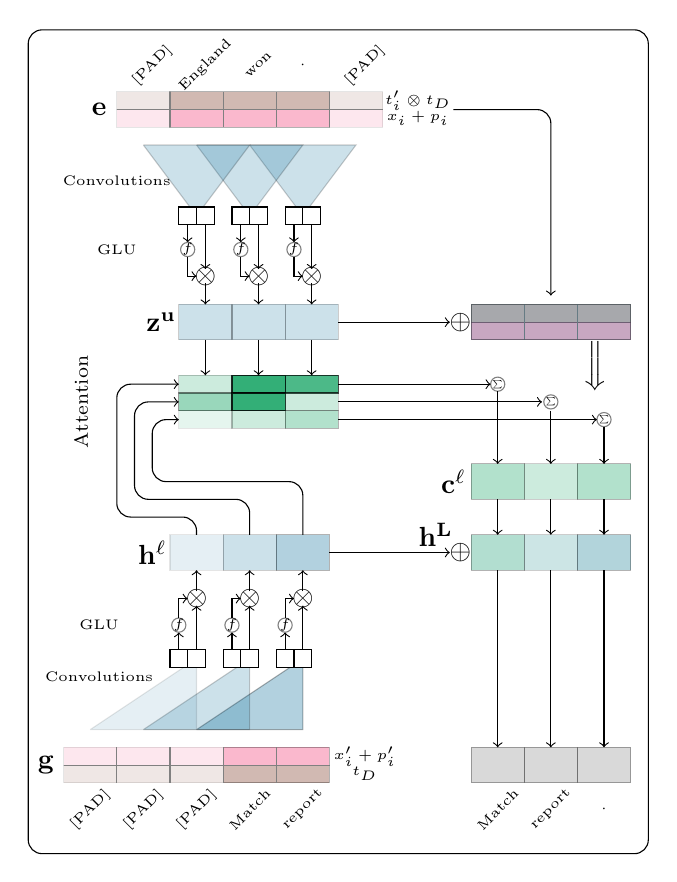
\begin{tikzpicture}[scale=0.45]
      
      \begin{scope}[shift={(0,0)}] 
        \draw [rounded corners=5pt] (-2.5,1.75) rectangle (15,-21.5);
        
        \draw [fill=sepia,opacity=0.1] (0,0) rectangle (1.5,-0.5);
        \draw [fill=sepia,opacity=0.3] (1.5,0) rectangle (6,-0.5);
        \draw [fill=sepia,opacity=0.1] (6,0) rectangle (7.5,-0.5);
        \draw [fill=orangered,opacity=0.1] (0,-0.5) rectangle (1.5,-1);
        \draw [fill=orangered,opacity=0.3] (1.5,-0.5) rectangle (6,-1);
        \draw [fill=orangered,opacity=0.1] (6,-0.5) rectangle (7.5,-1);
        
        \draw [gray] (0,-0.5) -- (7.5,-0.5);
        \draw [gray] (1.5,0) -- (1.5,-1);
        \draw [gray] (3,0) -- (3,-1);
        \draw [gray] (4.5,0) -- (4.5,-1);
        \draw [gray] (6,0) -- (6,-1);
        \node at (8.5,-0.75) {\tiny $x_i+p_i$};
        \node at (8.5,-0.25) {\tiny $t'_i \otimes t_D$};  
        \node at (-0.5,-0.5) {$\mathbf{e}$};

        \node at (1,0.75) {\tiny \rotatebox{45}{[PAD]}}; 
        \node at (2.5,0.75) {\tiny \rotatebox{45}{England}}; 
        \node at (4,0.75) {\tiny \rotatebox{45}{won}}; 
        \node at (5.25,0.75) {\tiny \rotatebox{45}{.}}; 
        \node at (7,0.75) {\tiny \rotatebox{45}{[PAD]}}; 
        
        % Convolution Part
        
        \node at (0,-2.5) {\tiny Convolutions};
        
        \draw [fill=midnightblue,opacity=0.2] (3.75,-1.5) -- (6.75, -1.5) -- (5.25, -3.5) -- (3.75,-1.5);
        \draw [fill=midnightblue,opacity=0.2] (2.25,-1.5) -- (5.25, -1.5) -- (3.75, -3.5) -- (2.25,-1.5);
        \draw [fill=midnightblue,opacity=0.2] (0.75,-1.5) -- (3.75, -1.5) -- (2.25, -3.5) -- (0.75,-1.5);
        
        \draw [fill=white,opacity=1] (1.75,-3.25) rectangle (2.75,-3.75);
        \draw [fill=white,opacity=1] (3.25,-3.25) rectangle (4.25,-3.75);
        \draw [fill=white,opacity=1] (4.75,-3.25) rectangle (5.75,-3.75);
        
        \draw (2.25,-3.25) -- (2.25,-3.75);
        \draw (3.75,-3.25) -- (3.75,-3.75);
        \draw (5.25,-3.25) -- (5.25,-3.75);
        
        % Gated Linear Unit

        \node at (0,-4.45) {\tiny GLU};
        
        \draw [->] (2,-3.75) -- (2,-4.25);
        \draw [gray] (2,-4.45) circle (0.2cm);
        \node at (2, -4.45) {\tiny $f$};
        \draw [->] (2.5,-3.75) -- (2.5,-5);
        \node at (2.5, -5.2) {$\otimes$};
        \draw [->] (2, -4.65) -- (2, -5.2) -- (2.25,-5.2);
        \draw [->] (2.5,-5.4) -- (2.5,-6);

        \draw [->] (3.5,-3.75) -- (3.5,-4.25);
        \draw [gray] (3.5, -4.45) circle (0.2cm);
        \node at (3.5, -4.45) {\tiny $f$};
        \draw [->] (4,-3.75) -- (4,-5);
        \node at (4,-5.2) {$\otimes$};
        \draw [->] (3.5,-4.65) -- (3.5,-5.2) -- (3.75,-5.2);
        \draw [->] (4,-5.4) -- (4,-6);

        \draw [->] (5,-3.75) -- (5,-4.25);
        \draw [gray] (5, -4.45) circle (0.2cm);
        \node at (5, -4.45) {\tiny $f$};
        \draw [->] (5.5,-3.75) -- (5.5,-5);
        \node at (5.5, -5.2) {$\otimes$};
        \draw [->] (5, -4.65) -- (5,-5.2) -- (5.25,-5.2);
        \draw [->] (5.5,-5.4) -- (5.5,-6);

        \draw [fill=midnightblue,opacity=0.2] (1.75,-6) rectangle (3.25,-7);
        \draw [fill=midnightblue,opacity=0.2] (3.25,-6) rectangle (4.75,-7);
        \draw [fill=midnightblue,opacity=0.2] (4.75,-6) rectangle (6.25,-7);
        \node at (1.25,-6.5) {$\mathbf{z^u}$};

        % Attention Part
        \node at (-1,-8.75) {\scriptsize \rotatebox{90}{Attention}}; 

        \draw [->] (2.5,-7) -- (2.5,-8);
        \draw [->] (4,-7) -- (4,-8);
        \draw [->] (5.5,-7) -- (5.5,-8);
        
        
        \draw [fill=forestgreen,opacity=0.2] (1.75,-8) rectangle (3.25,-8.5);
        \draw [fill=forestgreen,opacity=0.8] (3.25,-8) rectangle (4.75,-8.5);
        \draw [fill=forestgreen,opacity=0.7] (4.75,-8) rectangle (6.25,-8.5);
        \draw [fill=forestgreen,opacity=0.4] (1.75,-8.5) rectangle (3.25,-9);
        \draw [fill=forestgreen,opacity=0.8] (3.25,-8.5) rectangle (4.75,-9);
        \draw [fill=forestgreen,opacity=0.2] (4.75,-8.5) rectangle (6.25,-9);
        \draw [fill=forestgreen,opacity=0.1] (1.75,-9) rectangle (3.25,-9.5);
        \draw [fill=forestgreen,opacity=0.2] (3.25,-9) rectangle (4.75,-9.5);
        \draw [fill=forestgreen,opacity=0.3] (4.75,-9) rectangle (6.25,-9.5);

        % 
        \draw [fill=sepia,opacity=0.3] (10,-6) rectangle (14.5,-6.5);
        \draw [fill=orangered,opacity=0.3] (10,-6.5) rectangle (14.5,-7);
        \draw [gray] (11.5,-6) -- (11.5,-7);
        \draw [gray] (13,-6) -- (13,-7);
        \draw [fill=midnightblue,opacity=0.2] (10,-6) rectangle (14.5,-7);
        
        \draw [rounded corners=5pt,->] (9.5,-0.5) -- (12.25, -0.5) -- (12.25, -5.75);
        \draw [->] (6.25,-6.5) -- (9.4, -6.5);
        \node at (9.7,-6.5) {$\oplus$};
        % \node at (9.7,-6.5) {$\oplus$};
      \end{scope}

      \begin{scope}[shift={(-1.5,-19.5)}] 
        
        \draw [fill=sepia,opacity=0.1] (0,0) rectangle (4.5,0.5);
        \draw [fill=sepia,opacity=0.3] (4.5,0) rectangle (7.5,0.5);        
        \draw [fill=orangered,opacity=0.1] (0,0.5) rectangle (4.5,1);
        \draw [fill=orangered,opacity=0.3] (4.5,0.5) rectangle (7.5,1);

        \node at (0.75,-0.75) {\tiny \rotatebox{45}{[PAD]}}; 
        \node at (2.25,-0.75) {\tiny \rotatebox{45}{[PAD]}}; 
        \node at (3.75,-0.75) {\tiny \rotatebox{45}{[PAD]}}; 
        \node at (5.25,-0.75) {\tiny \rotatebox{45}{Match}}; 
        \node at (6.75,-0.75) {\tiny \rotatebox{45}{report}}; 
        

        \draw [gray] (0,0.5) -- (7.5,0.5);
        \draw [gray] (1.5,0) -- (1.5,1);
        \draw [gray] (3,0) -- (3,1);
        \draw [gray] (4.5,0) -- (4.5,1);
        \draw [gray] (6,0) -- (6,1);
        \node at (8.5,0.75) {\tiny $x'_i+p'_i$};
        \node at (8.5,0.25) {\tiny $t_D$};        
        \node at (-0.5,0.5) {$\mathbf{g}$};

        % Convolution Part
        
        \node at (1,3) {\tiny Convolutions};

        \draw [fill=midnightblue,opacity=0.3] (3.75,1.5) -- (6.75, 1.5) -- (6.75, 3.5) -- (3.75,1.5);
        \draw [fill=midnightblue,opacity=0.2] (2.25,1.5) -- (5.25, 1.5) -- (5.25, 3.5) -- (2.25,1.5);
        \draw [fill=midnightblue,opacity=0.1] (0.75,1.5) -- (3.75, 1.5) -- (3.75, 3.5) -- (0.75,1.5);
        
        \draw [fill=white,opacity=1] (3,3.25) rectangle (4,3.75);
        \draw [fill=white,opacity=1] (4.5,3.25) rectangle (5.5,3.75);
        \draw [fill=white,opacity=1] (6,3.25) rectangle (7,3.75);
        
        \draw (3.5,3.25) -- (3.5,3.75);
        \draw (5,3.25) -- (5,3.75);
        \draw (6.5,3.25) -- (6.5,3.75);
        
        % Gated Linear Unit
        \node at (1,4.45) {\tiny GLU};

        \draw [->] (3.25,3.75) -- (3.25,4.25);
        \draw [gray] (3.25, 4.45) circle (0.2cm);
        \node at (3.25, 4.45) {\tiny $f$};
        \draw [->] (3.75,3.75) -- (3.75,5);
        \node at (3.75, 5.2) {$\otimes$};
        \draw [->] (3.25, 4.65) -- (3.25, 5.2) -- (3.5,5.2);
        \draw [->] (3.75,5.4) -- (3.75,6);

        \draw [->] (4.75,3.75) -- (4.75,4.25);
        \draw [gray] (4.75, 4.45) circle (0.2cm);
        \node at (4.75, 4.45) {\tiny $f$};
        \draw [->] (5.25,3.75) -- (5.25,5);
        \node at (5.25, 5.2) {$\otimes$};
        \draw [->] (4.75, 4.65) -- (4.75,5.2) -- (5,5.2);
        \draw [->] (5.25,5.4) -- (5.25,6);

        \draw [->] (6.25,3.75) -- (6.25,4.25);
        \draw [gray] (6.25, 4.45) circle (0.2cm);
        \node at (6.25, 4.45) {\tiny $f$};
        \draw [->] (6.75,3.75) -- (6.75,5);
        \node at (6.75, 5.2) {$\otimes$};
        \draw [->] (6.25, 4.65) -- (6.25,5.2) -- (6.5,5.2);
        \draw [->] (6.75,5.4) -- (6.75,6);

        \draw [fill=midnightblue,opacity=0.1] (3,6) rectangle (4.5,7);
        \draw [fill=midnightblue,opacity=0.2] (4.5,6) rectangle (6,7);
        \draw [fill=midnightblue,opacity=0.3] (6,6) rectangle (7.5,7);
        
        \node at (2.5,6.5) {$\mathbf{h^{\ell}}$};

        % After Attention weights
        \draw [fill=forestgreen,opacity=0.3] (11.5,8) rectangle (13,9);
        \draw [fill=forestgreen,opacity=0.2] (13,8) rectangle (14.5,9);
        \draw [fill=forestgreen,opacity=0.3] (14.5,8) rectangle (16,9);     
        \draw [->] (12.25,8) -- (12.25,7);     
        \draw [->] (13.75,8) -- (13.75,7);     
        \draw [->] (15.25,8) -- (15.25,7); 
        \node at (11,8.5) {$\mathbf{c^{\ell}}$};

        \draw [fill=midnightblue!20!forestgreen,opacity=0.3] (11.5,6) rectangle (13,7);
        \draw [fill=midnightblue!60!forestgreen,opacity=0.2] (13,6) rectangle (14.5,7);
        \draw [fill=midnightblue!80!forestgreen,opacity=0.3] (14.5,6) rectangle (16,7);        
        \draw [->] (7.5,6.5) -- (10.9, 6.5);
        \node at (11.2,6.5) {$\oplus$}; 
        \node at (10.5,7) {$\mathbf{h^L}$};
        
        % Predict
        \draw [->] (12.25,6) -- (12.25,1); 
        \draw [fill=gray,opacity=0.3] (11.5,0) rectangle (13,1);
        \draw [->] (13.75,6) -- (13.75,1);     
        \draw [fill=gray,opacity=0.3] (13,0) rectangle (14.5,1);
        \draw [->] (15.25,6) -- (15.25,1);     
        \draw [fill=gray,opacity=0.3] (14.5,0) rectangle (16,1);
        
        \node at (12.25,-0.75) {\tiny \rotatebox{45}{Match}}; 
        \node at (13.75,-0.75) {\tiny \rotatebox{45}{report}}; 
        \node at (15.25,-0.75) {\tiny \rotatebox{45}{.}}; 
        

        % Connect to Attention
        \draw [rounded corners=5pt,->] (3.75,7) -- (3.75,7.5) -- (1.5, 7.5) -- (1.5, 11.25) -- (3.25, 11.25);
        \draw [rounded corners=5pt,->] (5.25,7) -- (5.25,8) -- (2, 8) -- (2, 10.75) -- (3.25, 10.75);
        \draw [rounded corners=5pt,->] (6.75,7) -- (6.75,8.5) -- (2.5, 8.5) -- (2.5, 10.25) -- (3.25, 10.25);
        % Predict using attention
        \draw [gray] (12.25,11.25) circle (0.2cm);
        \node at (12.25,11.25) {\fontsize{3}{5}\selectfont $\sum$};
        \draw [->] (7.75, 11.25) -- (12.05,11.25);
        \draw [->] (12.25, 11.05) -- (12.25,9);

        \draw [gray] (13.75,10.75) circle (0.2cm);
        \node at (13.75,10.75) {\fontsize{3}{5}\selectfont $\sum$};
        \draw [->] (7.75, 10.75) -- (13.5,10.75);
        \draw [->] (13.75, 10.5) -- (13.75,9);
        
        \draw [gray] (15.25,10.25) circle (0.2cm);
        \node at (15.25,10.25) {\fontsize{3}{5}\selectfont $\sum$};
        \draw [->] (7.75, 10.25) -- (15.05,10.25);
        \draw [->] (15.25, 10.05) -- (15.25,9);
        
        \node at (15,11.75) {$\Big\Downarrow$};
      \end{scope}
    \end{tikzpicture}
  }
  \vspace{-0.5cm}
  \caption{Topic-conditioned convolutional model for extreme
    summarization.}\label{fig:architecture}
\end{figure}

Unlike tasks like machine translation and paraphrase generation where
there is often a one-to-one semantic correspondence between source and
target words, document summarization must distill the content of the
document into a few important facts. This is even more challenging for
our task, where the compression ratio is extremely high, and pertinent
content can be easily missed.


%to distinguish content which is relevant for the
%summary from content which isn't. As such the challenges for extreme
%summarization are primarily in modeling long-range dependencies and
%recognizing pertinent content in the document.

Recently, a convolutional alternative to sequence modeling has been
proposed showing promise for machine translation
\cite{convenc_mt,convseq2seq} and story generation
\cite{fan-hier-gen}. We believe that convolutional architectures are
attractive for our summarization task for at least two
reasons. Firstly, contrary to recurrent networks which view the input
as a chain structure, convolutional networks can be stacked to
represent large context sizes. Secondly, hierarchical features can be
extracted over larger and larger contents, allowing to represent
long-range dependencies efficiently through shorter paths.

Our model builds on the work of \newcite{convseq2seq} who develop an
encoder-decoder architecture for machine translation with an attention
mechanism \cite{NIPS2015_5846} based exclusively on deep convolutional
networks. We adapt this model to our summarization task by allowing it
to recognize pertinent content (i.e.,~by foregrounding salient words
in the document).  In particular, we improve the convolutional encoder
by associating each word with a vector representing topic salience,
and the convolutional decoder by conditioning each word prediction on
the document topic vector.


% uses information about topical words in the document and the topic
% of the document to calibrate the modeling of long-range dependencies
% with the important content in the document for abstractive summary
% generation.

\paragraph{Model Overview}

At the core of our model is a simple convolutional block structure
that computes intermediate states based on a fixed number of input
elements. Our convolutional encoder (shown at the top of Figure
\ref{fig:architecture}) applies this unit across the document. We
repeat these operations in a stacked fashion to get a multi-layer
hierarchical representation over the input document where words at
closer distances interact at lower layers while distant words interact
at higher layers. The interaction between words through hierarchical
layers effectively captures long-range dependencies. 
% between distant
%words.% than when
%they are modelled with recurrent neural networks.

Analogously, our convolutional decoder (shown at the bottom of
Figure~\ref{fig:architecture}) uses the multi-layer convolutional
structure to build a hierarchical representation over what has been
predicted so far. Each layer on the decoder side determines useful
source context by attending to the encoder representation before it
passes its output to the next layer. This way the model remembers
which words it previously attended to and applies multi-hop attention
(shown at the middle of Figure \ref{fig:architecture}) per time
step. The output of the top layer is passed to a softmax classifier to
predict a distribution over the target vocabulary.


Our model assumes access to word and document topic
distributions. These can be obtained by any topic model, however we
use Latent Dirichlet Allocation (LDA; \citealt{Blei:2003:LDA}) in our
experiments; we pass the distributions obtained from LDA directly to
the network as additional input. This allows us to take advantage of
topic modeling without interfering with the computational advantages
of the convolutional architecture. The idea of capturing
document-level semantic information has been previously explored for
recurrent neural networks
\cite{mikolovZ12,Ghosh2016ContextualL,dieng-iclr17}, however, we are
not aware of any existing convolutional models.


\paragraph{Topic Sensitive Embeddings}

Let~$D$ denote a document consisting of a sequence of words $(w_1,
\ldots, w_m)$; we embed~$D$ into a distributional space $\mathbf{x} =
(x_1, \ldots, x_m)$ where $x_i \in \mathbb{R}^f$ is a column in
embedding matrix $M \in \mathbb{R}^{V\times f}$ (where $V$ is the
vocabulary size). We also embed the absolute word positions in the
document \mbox{$\mathbf{p} = (p_1, \ldots, p_m)$} where $p_i \in
\mathbb{R}^f$ is a column in position matrix $P \in
\mathbb{R}^{N\times f}$, and $N$ is the maximum number of
positions. Position embeddings have proved useful for convolutional
sequence modeling \cite{convseq2seq}, because, in contrast to RNNs,
they do not observe the temporal positions of words
\cite{D16-1248}. Let $t_D \in \mathbb{R}^{f'}$ be the topic
distribution of document~$D$ and $\mathbf{t'} = (t'_1, \ldots, t'_m)$
the topic distributions of words in the document (where $t'_i \in
\mathbb{R}^{f'}$). During encoding, we represent document~$D$ via
$\mathbf{e} = (e_1, \ldots, e_m)$, where~$e_i$ is:
\begin{align}
e_i = [(x_i+p_i);(t'_i\otimes t_D)] \in \mathbb{R}^{f+f'}, \label{eq:encoder}
\end{align}
\noindent and $\otimes$ denotes point-wise multiplication. The topic
distribution $t'_i$ of word $w_i$ essentially captures how topical the
word is in itself (local context), whereas the topic
distribution~$t_D$ represents the overall theme of the document
(global context). The encoder essentially enriches the context of the
word with its topical relevance to the document.


For every output prediction, the decoder estimates representation
$\mathbf{g} = (g_1, \ldots, g_n)$ for previously predicted words
$(w'_1, \ldots, w'_n)$ where $g_i$ is:
\begin{align}
g_i = [(x'_i+p'_i);t_D] \in \mathbb{R}^{f+f'}, \label{eq:decoder}
\end{align}
\noindent $x'_i$ and $p'_i$ are word and position embeddings of
previously predicted word~$w'_i$, and $t_D$ is the topic distribution
of the input document. Note that the decoder does not use the topic
distribution of~$w'_i$ as computing it on the fly would be
expensive. However, every word prediction is conditioned on the topic
of the document, enforcing the summary to have the same theme as the
document.

% We propose to use word topic information for local context and
% document topic to model global context.

\paragraph{Multi-layer Convolutional Structure}

Each convolution block, parametrized by $W \in \mathbb{R}^{2d\times
  kd}$ and $b_w \in \mathbb{R}^{2d}$, takes as input $X \in
\mathbb{R}^{k\times d}$ which is the concatenation of $k$ adjacent
elements embedded in a~$d$ dimensional space, applies one dimensional
convolution and returns an output element $Y \in \mathbb{R}^{2d}$. We
apply Gated Linear Units (GLU, $v:\mathbb{R}^{2d} \rightarrow
\mathbb{R}^{d}$, \citeauthor{pmlr-v70-dauphin17a}
\citeyear{pmlr-v70-dauphin17a}) on the output of the convolution
$Y$. Subsequent layers operate over the $k$ output elements of the
previous layer and are connected through residual connections
\cite{He2016DeepRL} to allow for deeper hierarchical
representation. We denote the output of the $\ell$th layer as
$\mathbf{h^{\ell}} = (h^{\ell}_1, \ldots, h^{\ell}_n)$ for the decoder
network, and $\mathbf{z^{\ell}} = (z^{\ell}_1, \ldots, z^{\ell}_m)$
for the encoder network.

\paragraph{Multi-hop Attention}

Our encoder and decoder are tied to each other through a multi-hop
attention mechanism. For each decoder layer $\ell$, we compute the
attention $a^{\ell}_{ij}$ of state $i$ and source element $j$ as:
\begin{align}
a^{\ell}_{ij} = \frac{\mbox{exp}(d^{\ell}_i \cdot z^u_j)}{\sum^m_{t=1} \mbox{exp}(d^{\ell}_i \cdot z^u_t)}, \label{eq:attention}
\end{align}
\noindent where $d^{\ell}_i = W^{\ell}_dh^{\ell}_i+b^{\ell}_i+g_i$ is
the decoder state summary combining the current decoder state
$h^{\ell}_i$ and the previous output element embedding $g_i$. The
vector $\mathbf{z^u}$ is the output from the last encoder layer
$u$. The conditional input $c^{\ell}_i$ to the current decoder layer
is a weighted sum of the encoder outputs as well as the input element
embeddings $e_j$:
\begin{align}
c^{\ell}_i = \sum^m_{j=1} a^{\ell}_{ij}(z^u_j+e_j). \label{eq:decinput}
\end{align}

The attention mechanism described here performs multiple attention
``hops'' per time step and considers which words have been previously
attended to. It is therefore different from single-step attention in
recurrent neural networks \cite{bahdanau-arxiv14}, where the attention
and weighted sum are computed over $\mathbf{z^u}$ only.

Our network uses multiple linear layers to project between the
embedding size $(f+f')$ and the convolution output size $2d$. They are
applied to~$\mathbf{e}$ before feeding it to the encoder, to the final
encoder output $\mathbf{z^u}$, to all decoder layers~$\mathbf{h^{\ell}}$
for the attention score computation, and to the final decoder output
$\mathbf{h^L}$ before the softmax.  We pad the input with~$k-1$ zero
vectors on both left and right side to ensure that the output of the
convolutional layers matches the input length. During decoding, we
ensure that the decoder does not have access to future information; we
start with $k$~zero vectors and shift the covolutional block to the
right after every prediction. The final decoder output $\mathbf{h^L}$
is used to compute the distribution over the target vocabulary $T$ as:
%
\begin{align}
  p(y_{i+1}|y_1,\ldots,y_i,D,t_D,\mathbf{t'}) = & \\
& \hspace*{-2cm}\mbox{softmax}(W_oh^L_i+b_o) \in \mathbb{R}^T. \label{eq:prediction}
\end{align}
%
We use layer normalization and weight initialization to
stabilize learning. 


Our topic-enhanced model calibrates long-range dependencies with
globally salient content. As a result, it provides a better
alternative to vanilla convolutional sequence models
\cite{convseq2seq} and RNN-based summarization models \cite{see-acl17}
for capturing cross-document inferences and paraphrasing.  At the same
time it retains the computational advantages of convolutional
models. Each convolution block operates over a fixed-size window of
the input sequence, allowing for simultaneous encoding of the input,
ease in learning due to the fixed number of non-linearities and
transformations for words in the input sequence.
%In
%contrast, RNNs are constrained by temporal dependencies in modeling
%long-range dependencies. Figure \ref{fig:architecture} gives an
%overview of our model.



% We refer the reader to \newcite{convseq2seq} for
% convolutional sequence modeling. Figure \ref{fig:architecture} gives
% an overview of our model.

%%% Local Variables:
%%% mode: latex
%%% TeX-master: "extreme-sum"
%%% End:



% Exp Setup and Evaluations
\section{Experimental Setup}
\label{sec:setup}

In this section we present our experimental setup for assessing the
performance of our \textbf{T}opic-aware \textbf{Conv}olutional
\textbf{S}equence \textbf{to} \textbf{S}equence model which we call
\textsc{T-ConvS2S} for short.  We discuss implementation details and
present the systems used for comparison with our approach.



\paragraph{Comparison Systems} 
We report results with various systems which were all trained on the
XSum dataset to generate a one-line summary given an input news
article.  We compared \mbox{\textsc{T-ConvS2S}} against three
extractive systems: a baseline which randomly selects a sentence from
the input document (\textsc{random}), a baseline which simply selects
the leading sentence from the document (\textsc{lead}), and an oracle
which selects a single-best sentence in each document
(\textsc{ext-oracle}). The latter is often used as an upper bound for
extractive methods. We also compared our model against the RNN-based
abstractive systems introduced by \newcite{see-acl17}. In particular,
we experimented with an attention-based sequence to sequence model
(\textsc{Seq2Seq}), a pointer-generator model which allows to copy
words from the source text (\textsc{PtGen}), and a pointer-generator
model with a coverage mechanism to keep track of words that have been
summarized (\textsc{PtGen-Covg}). Finally, we compared our model
against the vanilla convolution sequence to sequence model
(\textsc{ConvS2S}) of \newcite{convseq2seq}.



\paragraph{Model Parameters and Optimization} 

We did not anonymize entities but worked on a lowercased version of
the XSum dataset. During training and at test time the input document
was truncated to 400~tokens and  the length of the summary limited to
90~tokens.

The LDA model \cite{Blei:2003:LDA} was trained on XSum documents
(training portion). We therefore obtained for each word a probability
distribution over topics which we used to estimate $\mathbf{t'}$; the
topic distribution $t_D$ can be inferred for any new document, at
training and test time. We explored several LDA configurations on
held-out data, and obtained best results with~512
topics. Table~\ref{fig:lda-topics} shows some of the topics learned by
the LDA model.

%Once the LDA model is trained,
%we obtain a probability distribution over topics for each word in the
%training documents which we use to estimate $\mathbf{t'}$ and can
%infer the topic distribution $t_D$ for any new document, during both
%the training and test times.

For \textsc{Seq2Seq}, \textsc{PtGen} and \textsc{PtGen-Covg}, we used
the best settings reported on the CNN and DailyMail data
\cite{see-acl17}.\footnote{We used the code available at
  \url{https://github.com/abisee/pointer-generator}.}  All three
models had 256~dimensional hidden states and 128~dimensional word
embeddings. They were trained using Adagrad \cite{Duchi:2011} with
learning rate~0.15 and an initial accumulator value of~0.1. We used
gradient clipping with a maximum gradient norm of~2, but did not use
any form of regularization.  We used the loss on the validation set to
implement early stopping. 
%\textsc{Seq2Seq} takes around 4 days to
%train whereas \textsc{PtGen} and \textsc{PtGen-Covg} take around 2
%days each.\shaycomment{I am concerned that reviewers will claim that
%  you optimized hyperparameters on XSum for your model, but didn't do
%  the same for See's model.}

\begin{table}[t!]
  \center{\fontsize{10}{12}\selectfont % \footnotesize
    \begin{tabular}{@{}l@{\hspace{1.9ex}}p{6.7cm} }
      \thickhline 
      
      {T1:}& charge, court, murder, police, arrest, guilty, sentence, boy, bail, space, crown, trial \\
      
      {T2:}& church, abuse, bishop, child, catholic, gay, pope, school, christian, priest, cardinal \\
      
      {T3:}& council, people, government, local, housing, home, house, property, city, plan, authority \\
      
      {T4:}& clinton, party, trump, climate, poll, vote, plaid, election, debate, change, candidate, campaign\\
      
      {T5:}& country, growth, report, business, export, fall, bank, security, economy, rise, global, inflation\\
      
      {T6:}& hospital, patient, trust, nhs, people, care, health, service, staff, report, review, system, child\\

      \thickhline
    \end{tabular}     
  }
  \caption{Example topics learned by the LDA model on XSum documents
(training portion).}\label{fig:lda-topics}
\end{table}

For \textsc{ConvS2S}\footnote{We used the code available at
  \url{https://github.com/facebookresearch/fairseq-py}.} and
\textsc{T-ConvS2S}, we used 512 dimensional hidden states and 512
dimensional word and position embeddings. We trained our convolutional
models with Nesterov's accelerated gradient method
\cite{Sutskever:2013} using a momentum value of 0.99 and renormalized
gradients if their norm exceeded~0.1 \cite{Pascanu:2013}. We used a
learning rate of 0.10 and once the validation perplexity stopped
improving, we reduced the learning rate by an order of magnitude after
each epoch until it fell below~$10^{-4}$. We also applied a dropout
of~0.2 to the embeddings, the decoder outputs and the input of the
convolutional blocks. Gradients were normalized by the number of
non-padding tokens per mini-batch. We also used weight normalization
for all layers except for lookup tables.

All neural models, including ours and those based on RNNs \cite{see-acl17}
had a vocabulary of 50,000 words and were trained on a single Nvidia
M40 GPU with a batch size of~32 sentences.  Summaries at test time
were obtained using beam search (with beam size 10).

\section{Results}
\label{sec:results}


\paragraph{Automatic Evaluation} 

We report results using automatic metrics in Table~\ref{tab:rouge}.
We evaluated summarization quality using F$_1$ $\mbox{ROUGE}$
\cite{rouge}. Unigram and bigram overlap ($\mbox{ROUGE-1}$ and
$\mbox{ROUGE-2}$) are a proxy for assessing informativeness and the
longest common subsequence ($\mbox{ROUGE-L}$) represents
fluency.\footnote{We used \texttt{pyrouge} to compute all ROUGE
  scores, with parameters ``-a -c 95 -m -n 4 -w 1.2.''}



On the XSum dataset, \textsc{Seq2Seq} outperforms the \textsc{lead}
and \textsc{random} baselines by a large margin. \textsc{PtGen}, a
\textsc{Seq2Seq} model with a ``copying'' mechanism outperforms
\textsc{ext-oracle}, a ``perfect'' extractive system on ROUGE-2 and
ROUGE-L. This is in sharp contrast to the performance of these models
on CNN/DailyMail \cite{see-acl17} and  Newsroom datasets
\cite{newsroom-naacl18}, where they fail to outperform the
\textsc{lead}. The result provides further evidence that XSum is a
good testbed for abstractive summarization. \textsc{PtGen-Covg}, the
best performing abstractive system on the CNN/DailyMail datasets, does
not do well.  We believe that the coverage mechanism is more useful
when generating multi-line summaries and is basically redundant for
extreme summarization. 

\begin{table}[t]
  \begin{center}{\fontsize{8.5}{11}\selectfont %\footnotesize
  \begin{tabular}{ l | c c c }
    \thickhline
    Models & R1 & R2 & RL \\ \thickhline
    % \multicolumn{10}{c}{\textbf{Test Set (11334)}} \\ \hline
    Random & 15.16 & 1.78 & 11.27 \\ 
    \textsc{lead} & 16.30 & 1.60 & 11.95 \\ 
    \textsc{ext-oracle} & 29.79 & 8.81 & 22.66 \\ \hline
    \textsc{Seq2Seq} &  28.42 & 8.77 &  22.48 \\
    \textsc{PtGen} & 29.70 & 9.21 & 23.24 \\ 
    \textsc{PtGen-Covg} & 28.10 & 8.02 & 21.72 \\ 
    % \textsc{Transformer} & 28.63 & 9.58 & 23.29 \\ 
    \hline
    \textsc{ConvS2S} & 31.27 & 11.07 & 25.23 \\  % ppl drops to 23.4
    \textsc{T-ConvS2S} (enc$_{t'}$) & 31.71 & 11.38 & 25.56 \\
    \textsc{T-ConvS2S} (enc$_{t'}$, dec$_{t_D}$) & 31.71 & 11.34 & 25.61 \\
    \textsc{T-ConvS2S} (enc$_{(t',t_D)}$) & 31.61 & 11.30 & 25.51 \\
    \textsc{T-ConvS2S} (enc$_{(t',t_D)}$, dec$_{t_D}$)  & \textbf{31.89} & \textbf{11.54} & \textbf{25.75} \\ \thickhline % ppl drops to 23.04
    
    % \multicolumn{4}{c}{Weak Upper Bound} \\ \hline
    % Title  & 35.8 & 13.6 & 28.7 \\ \hline
  \end{tabular}
  }\end{center}
\caption{ROUGE results on  XSum test set. We report \mbox{ROUGE-1} (R1), ROUGE-2
  (R2), and ROUGE-L (RL) F$_1$  scores. Extractive systems are in the
  upper block, RNN-based   abstractive systems are in the middle block,
  and convolutional    abstractive systems are in the bottom
  block. \label{tab:rouge}} 
\end{table}

\begin{table}
  \begin{center}{\fontsize{8.5}{11}\selectfont % \footnotesize
  \begin{tabular}{ l | c c c c } 
    \thickhline
    \multirow{2}{*}{Models} & \multicolumn{4}{c}{\% of novel n-grams in generated summaries}  \\
    & unigrams & bigrams & trigrams & 4-grams  \\ \thickhline 
    \textsc{lead} & 0.00 & 0.00 & 0.00 & 0.00 \\
    \textsc{ext-oracle} & 0.00 & 0.00 & 0.00 & 0.00 \\
    % \textsc{Seq2Seq} & 36.66 & 82.17 & 95.58 & 98.63  \\
    \textsc{PtGen} & 27.40 & 73.33 & 90.43 & 96.04 \\ 
    % \textsc{PtGen-Covg} & 25.71 & 70.76 & 88.87 & 95.24 \\ \hline
    \textsc{ConvS2S} & \textbf{31.26} & \textbf{79.50} & \textbf{94.28} & \textbf{98.10}\\
    \textsc{T-ConvS2S}  & 30.73 & 79.18 & 94.10 & 98.03 \\ \hline
    \textsc{gold} & 35.76 & 83.45  & 95.50  & 98.49 \\ \thickhline
  \end{tabular}}
  \end{center}
  \caption{Proportion of novel $n$-grams in summaries generated by various models on the XSum test set.
    \label{tab:novelngram-xsum-models}}
\end{table}

\begin{table*}[t!]
  \center{ \footnotesize
    \begin{tabular}{l p{10.5cm} l}
      \thickhline 
      
      % 4306
      \textsc{ext-oracle} &Caroline Pidgeon is the Lib Dem candidate, Sian Berry will contest the election for the Greens and UKIP has chosen its culture spokesman Peter Whittle. &[34.1, 20.5, 34.1]\\
            
      {\textsc{PtGen}} & UKIP leader \textcolor{red}{Nigel Goldsmith} has been \textcolor{red}{elected} as the \textcolor{red}{new mayor of London} to elect a new conservative MP. &[45.7, 6.1, 28.6]  \\
      
      {\textsc{ConvS2S}}&  London mayoral candidate \textcolor{midnightblue}{Zac Goldsmith} has been \textcolor{red}{elected} as the \textcolor{red}{new mayor of London}.& [53.3, 21.4, 26.7]  \\

      {\textsc{T-ConvS2S}}& Former London mayoral candidate \textcolor{midnightblue}{Zac Goldsmith} has been \textcolor{midnightblue}{chosen to stand} in \textcolor{midnightblue}{the London mayoral election}. &[50.0, 26.7, 37.5] \\
      
      {\textsc{gold}}& \textcolor{midnightblue}{Zac Goldsmith} will \textcolor{midnightblue}{contest} the 2016 \textcolor{midnightblue}{London mayoral election} for the conservatives, it has been announced. \\
      
      {Questions}& (1) {Who will \textcolor{midnightblue}{contest} for
        the conservatives?} (\textcolor{midnightblue}{Zac
        Goldsmith})\\
 &  (2) {For what election will he/she contest?} (\textcolor{midnightblue}{The London mayoral election}) \\
            
      \hline
      % 4385
      {\textsc{ext-oracle}} &North-east rivals Newcastle are the only team below them in the Premier League table. &[35.3, 18.8, 35.3] \\
            
      {\textsc{PtGen}} &Sunderland have \textcolor{red}{appointed} former \textcolor{midnightblue}{Sunderland boss} \textcolor{midnightblue}{Dick Advocaat} as manager at the end of the season to sign a new deal. &[45.0, 10.5, 30.0] \\
      
      {\textsc{ConvS2S}} &Sunderland have \textcolor{red}{sacked} \textcolor{midnightblue}{manager} \textcolor{midnightblue}{Dick Advocaat} after less than three months in charge. &[25.0, 6.7, 18.8] \\

      {\textsc{T-ConvS2S}}& \textcolor{midnightblue}{Dick Advocaat} has \textcolor{midnightblue}{resigned} as \textcolor{midnightblue}{Sunderland manager} until the end of the season.& [56.3, 33.3, 56.3] \\
      
      {\textsc{gold}} &\textcolor{midnightblue}{Dick Advocaat} has \textcolor{midnightblue}{resigned} as \textcolor{midnightblue}{Sunderland boss}, with the team yet to win in the Premier League this season. \\
      
      Questions& (1) {Who has \textcolor{midnightblue}{resigned}?}
      (\textcolor{midnightblue}{Dick Advocaat}) \\& (2) {From what post has he/she resigned?} (\textcolor{midnightblue}{Sunderland boss}) \\
            
      \hline
      
      % 9590 
      {\textsc{ext-oracle}}& The Greater Ardoyne residents collective (GARC) is protesting against an agreement aimed at resolving a long-running dispute in the area. &[26.7, 9.3, 22.2]  \\

      {\textsc{PtGen}} &A residents' group has been granted permission for GARC to hold a parade on \textcolor{red}{the outskirts of Crumlin, County Antrim}. &[28.6, 5.0, 28.6] \\

      {\textsc{ConvS2S}} &A protest has been held in the \textcolor{midnightblue}{Republic of Ireland} calling for \textcolor{red}{an end to parading} parading in \textcolor{midnightblue}{North Belfast}. &[42.9, 20.0, 33.3] \\

      {\textsc{T-ConvS2S}}& A protest has been held in \textcolor{midnightblue}{North Belfast} over a protest against \textcolor{midnightblue}{the Orange Order} in \textcolor{midnightblue}{North Belfast}.& [45.0, 26.3, 45.0] \\

      {\textsc{gold}} &Church leaders have appealed to a nationalist residents' group to call off a protest against \textcolor{midnightblue}{an Orange Order parade} in \textcolor{midnightblue}{North Belfast}. \\

      Questions &(1) {Where is the protest supposed to happen?}
      (\textcolor{midnightblue}{North Belfast}) \\ 
&(2) {What are they protesting against?} (\textcolor{midnightblue}{An Orange Order parade}) \\
      \thickhline

    \end{tabular}     
  }
  \caption{Example output summaries on the XSum test set with [ROUGE-1,
    ROUGE-2 and ROUGE-L] scores, goldstandard reference, and
    corresponding questions. Words highlighted in blue are either the
    right answer or constitute appropriate context for inferring it;
    words in red lead to the wrong
    answer. }\label{tab:erroranalysis}
\end{table*}


\textsc{ConvS2S}, the convolutional variant of \textsc{Seq2Seq},
significantly outperforms all \mbox{RNN-based} abstractive systems. We
hypothesize that its superior performance stems from the ability to
better represent document content (i.e.,~by capturing long-range
dependencies).
% for abstractive summarization. \shaycomment{you keep
%  mentioning long-range dependencies, but do you ever show that this
%  is what we tackle?}
Table~\ref{tab:rouge} shows several variants of \textsc{T-ConvS2S}
including an encoder network enriched with information about how
topical a word is on its own (enc$_{t'}$) or in the document
(enc$_{(t',t_D)}$).  We also experimented with various decoders by
conditioning every prediction on the topic of the document, basically
encouraging the summary to be in the same theme as the document
(dec$_{t_D}$) or letting the decoder decide the theme of the
summary. Interestingly, all four \textsc{T-ConvS2S} variants
outperform \textsc{ConvS2S}. \textsc{T-ConvS2S} performs best when
both encoder and decoder are constrained by the document topic
(enc$_{(t',t_D)}$,dec$_{t_D}$). In the remainder of the paper, we
refer to this variant as \textsc{T-ConvS2S}.

We further assessed the extent to which various models are able to
perform rewriting by generating genuinely abstractive
summaries. Table~\ref{tab:novelngram-xsum-models} shows the proportion
of novel $n$-grams for \textsc{lead}, \textsc{ext-oracle},
\textsc{PtGen}, \textsc{ConvS2S}, and \textsc{T-ConvS2S}.  As can be
seen, the convolutional models exhibit the highest proportion of novel
$n$-grams. We should also point out that the summaries being evaluated
have on average comparable lengths; the summaries generated by
\textsc{PtGen} contain 22.57 words, those generated by
\textsc{ConvS2S} and \textsc{T-ConvS2S} have 20.07 and 20.22 words,
respectively, while \textsc{gold} summaries are the longest with~23.26
words.  Interestingly, \textsc{PtGen} trained on XSum only copies 4\%
of 4-grams in the source document, 10\% of trigrams, 27\% of bigrams,
and 73\% of unigrams. This is in sharp contrast to \textsc{PtGen}
trained on CNN/DailyMail exhibiting mostly extractive patterns; it
copies more than 85\% of 4-grams in the source document, 90\% of
trigrams, 95\% of bigrams, and 99\% of unigrams \cite{see-acl17}. This
result further strengthens our hypothesis that XSum is a good testbed
for abstractive methods.

% is able to calibrate its document
%modeling with the pertinent content in the document for abstractive
%summarization and the decoder (dec$_{t_D}$) is guided towards
%generating summaries on the same topic as the document. 


\paragraph{Human Evaluation}
In addition to automatic evaluation using ROUGE which can be
misleading when used as the only means to assess the informativeness
of summaries \cite{schluter:2017:EACLshort}, we also evaluated system
output by eliciting human judgments in two ways. 

In our first experiment, participants were asked to compare summaries
produced from the \textsc{ext-oracle} baseline, \textsc{PtGen}, the
best performing system of \citet{see-acl17}, \textsc{ConvS2S}, our
topic-aware model \textsc{T-ConvS2S}, and the human-authored gold
summary (\textsc{gold}). We did not include extracts from the
\textsc{lead} as they were significantly inferior to other models. 


The study was conducted on the Amazon Mechanical Turk platform using
\textit{Best-Worst Scaling} (BWS; \citealt{louviere1991best,
  louviere2015best}), a less labor-intensive alternative to paired
comparisons that has been shown to produce more reliable results than
rating scales \cite{bestworstscaling}. Participants were presented
with a document and summaries generated from two out of five systems
and were asked to decide which summary was \textit{better} and which one
was \textit{worse} in order of informativeness (does the summary
capture important information in the document?) and fluency (is the
summary written in well-formed English?). Examples of system summaries
are shown in Table~\ref{tab:erroranalysis}.  We randomly selected
50~documents from the XSum test set and compared all possible
combinations of two out of five systems for each document. We
collected judgments from three different participants for each
comparison. The order of summaries was randomized per document and the
order of documents per participant.

\begin{table}[t]
  \center{\small
    \begin{tabular}{lrc}
      \thickhline
      Models  & Score & QA\\ \hline
      \textsc{ext-oracle} &  -0.121 & 15.70\\
      \textsc{PtGen} & -0.218& 21.40 \\
      \textsc{ConvS2S}  &
      -0.130 & 30.90 \\
      \textsc{T-ConvS2S} & \textbf{0.037} & \textbf{46.05}\\ \hline
      \textsc{gold} & 0.431 & 97.23\\
      \thickhline
    \end{tabular}}
  \caption{System ranking according to human judgments  and QA-based
    evaluation.\label{tab:heval-pref}}
\end{table}

The score of a system was computed as the percentage of times it was
chosen as best minus the percentage of times it was selected as
worst. The scores range from -1 (worst) to 1 (best) and are shown in
Table~\ref{tab:heval-pref}. Perhaps unsurprisingly human-authored
summaries were considered best, whereas, \textsc{T-ConvS2S} was ranked
2nd followed by \textsc{ext-oracle} and
\textsc{ConvS2S}. \textsc{PtGen} was ranked worst with the lowest
score of $-0.218$. We carried out pairwise comparisons between all
models to assess whether system differences are statistically
significant. \textsc{gold} is significantly different from all other
systems and \textsc{T-ConvS2S} is significantly different from
\textsc{ConvS2S} and \textsc{PtGen} (using a one-way ANOVA with
posthoc Tukey HSD tests; $p < 0.01$). All other differences are not
statistically significant.


%\shaycomment{make sure all tense
%  is consistent in the experiments section. you say sometimes was
%  ranked, then is ranked, etc.}

%\begin{table}[t]
%  \center{\footnotesize
%    \begin{tabular}{|@{~}l@{~~}| c@{~~} c@{~~} c@{~~} c@{~~} |c@{~}| } 
%      \hline
%      Models & \textsc{\scriptsize ext-oracle} & \textsc{\scriptsize PtGen} & \textsc{\scriptsize  ConvS2S} & \textsc{\scriptsize T-ConvS2S} & \textsc{\scriptsize gold} \\ \hline
%      QA & 15.70 & 21.40 & 30.90 & \textbf{46.05} & 97.23 \\
%      \hline
%    \end{tabular}}
%  \caption{QA-based evaluation. The row QA shows the percentage of questions
%    that participants answered correctly by reading system summaries.\label{tab:heval-qa}}
%\end{table}
%



For our second experiment we used a question-answering (QA) paradigm
\cite{Clarke:Lapata:2010,narayan-rank18} to assess the degree to which
the models retain key information from the document. We used the same
50 documents as in our first elicitation study.  We wrote two
fact-based questions per document, just by reading the summary, under
the assumption that it highlights the most important content of the
news article. Questions were formulated so as not to reveal answers to
subsequent questions.  We created 100~questions in total (see
Table~\ref{tab:erroranalysis} for examples). Participants read the
output summaries and answered the questions as best they could without
access to the document or the gold summary. The more questions can be
answered, the better the corresponding system is at summarizing the
document as a whole.  Five participants answered questions for each
summary.

We followed the scoring mechanism introduced in
\newcite{Clarke:Lapata:2010}. A correct answer was marked with a score
of one, partially correct answers with a score of~0.5, and zero
otherwise. The final score for a system is the average of all its
question scores. Answers again were elicited using Amazon's Mechanical
Turk crowdsourcing platform. We uploaded the data in batches (one
system at a time) to ensure that the same participant does not
evaluate summaries from different systems on the same set of
questions.

%Example questions are given in
%Figure~\ref{fig:erroranalysis}.

% Example questions are given in Figure~\ref{fig:erroranalysis}. Subjects
% were shown summaries from three systems: the \textsc{Lead} baseline,
% the abstractive system of \newcite{see-acl17}, and \refresh.




%\paragraph{Human Evaluation: System Ranking}

 
%\paragraph{Human Evaluation: Question Answering}

Table~\ref{tab:heval-pref} shows the results of the QA
evaluation. Based on summaries generated by \mbox{\textsc{T-ConvS2S}},
participants can answer $46.05\%$ of the questions
correctly. Summaries generated by \textsc{ConvS2S}, \textsc{PtGen} and
\textsc{ext-oracle} provide answers to $30.90\%$, $21.40\%$, and
$15.70\%$ of the questions, respectively. Pairwise differences between
systems are all statistically significant ($p < 0.01$) with the
exception of \textsc{PtGen} and \textsc{ext-oracle}.
\textsc{ext-oracle} performs poorly on both QA and rating
evaluations. The examples in Table~\ref{tab:erroranalysis} indicate
that \textsc{ext-oracle} is often misled by selecting a sentence with
the highest ROUGE (against the gold summary), but ROUGE itself does
not ensure that the summary retains the most important information
from the document.  The QA evaluation further emphasizes that in order
for the summary to be felicitous, information needs to be embedded in
the appropriate context. For example, \textsc{ConvS2S} and
\textsc{PtGen} will fail to answer the question ``Who has resigned?''
(see Table~\ref{tab:erroranalysis} second block) despite containing
the correct answer ``Dick Advocaat'' due to the wrong
context. \mbox{\textsc{T-ConvS2S}} is able to extract
important entities from the document with the right theme.

%Our analysis suggests that ROUGE should
%not be the only criteria to evaluate summarization systems, it should
%always be complemented with human evaluations.

%The question answering evaluation not only judges if the summary
%retains the main information from the document, but it also 



% A: "LEAD",
% B: "EXT-Oracle"
% C: "PTGen"
% D: "ConvS2S"
% E: "T-ConvS2S"
% 6: "GOLD"

%         Tukey HSD
% Q statistic        Tukey HSD
% p-value        Tukey HSD
% inferfence
% A vs B        1.7924        0.7769044        insignificant
% A vs C        5.1981        0.0032943        ** p<0.01
% A vs D        10.8742        0.0010053        ** p<0.01
% A vs E        19.5974        0.0010053        ** p<0.01
% A vs F        50.5470        0.0010053        ** p<0.01
% B vs C        3.4056        0.1536003        insignificant
% B vs D        9.0817        0.0010053        ** p<0.01
% B vs E        17.8050        0.0010053        ** p<0.01
% B vs F        48.7545        0.0010053        ** p<0.01
% C vs D        5.6761        0.0010053        ** p<0.01
% C vs E        14.3993        0.0010053        ** p<0.01
% C vs F        45.3489        0.0010053        ** p<0.01
% D vs E        8.7232        0.0010053        ** p<0.01
% D vs F        39.6728        0.0010053        ** p<0.01
% E vs F        30.9496        0.0010053        ** p<0.01




%\shashi{Anything else?}

%% We also found that ConS2s and TCon sec seems to get entities right. 
%% rEPEATITION, PTGEN IN CONV COULD HELP, WITHPOUT Copy MECHANISM


% May be T-Conv more factually correct than other. See this. Find other example.

% Abs methods might have correct answer but some wrong info, that is then causes difficulties to answer by users. (Find an example in support of this). However, ext always fluent, is found answer it will be correct.

% T-ConvS2s successfull achieves full name but fails to answer becuase misses the right context. But that is not the case with ext system.

% TConVseq or convs2s fails because does not get proper context: Despite of capturing the named entity. PTGen often find wron combo.

% [4306]Who will be the conservative contestant?
% 5 [1, 0, 0, 0, 0] T-ConvS2S 0.2
% 5 [0, 0, 0, 0, 0] LEAD 0.0
% 5 [1, 0, 1, 1, 1] GOLD 0.8
% 5 [0, 0, 0, 0, 0] PTGen 0.0
% 5 [0, 0, 0, 0, 0] EXT-Oracle 0.0
% 5 [0, 0, 0, 0, 0] ConvS2S 0.0

% [4385]Who has resigned?
% 5 [1, 1, 1, 1, 1] T-ConvS2S 1.0
% 5 [0, 0, 0, 0, 0] LEAD 0.0
% 5 [1, 1, 1, 1, 1] GOLD 1.0
% 5 [0, 0, 0, 0, 0] PTGen 0.0
% 5 [0, 0, 0, 0, 0] EXT-Oracle 0.0
% 5 [0, 1, 1, 0, 0] ConvS2S 0.4


%% Age etc is still a problem for all the model.

%% T-ConvS2S
%% the ska band , bradbury , has died at the age of 77 , the band has announced .
%% [1353]At what age did he die? A1GV0UZU0T2ORS
%% Candidate Answer: 77
%% Reference Answer: 62


%% Match reports
%% 2783   38782795 

% Position in RNN shown to learn by itlesf. \cite{D16-1248}
% Compare with seq2seq abssum models: We don't add position embed to seq2seq. No point, people have shown they already learn that in their neurons.


%%% Local Variables:
%%% mode: latex
%%% TeX-master: "extreme-sum"
%%% End:

% \begin{table}
%   \begin{center}{\footnotesize
%   \begin{tabular}{ l | c c c } 
%     % \multicolumn{4}{c}{\textsc{NewsRoom-Abstractive} Dataset} \\
%     \thickhline
%     Models & R1 & R2 & RL \\ \thickhline 
%     \multicolumn{4}{c}{\textsc{development set}} \\ \hline 
%     \textsc{lead-3} & 13.69 & 2.42 & 11.24 \\
%     % Fragments &  73.43 & 47.66 & 73.43 \\ 
%     TextRank & 13.54 & 1.88 & 10.46 \\
%     Abs-N & 6.21 & 1.07 & 5.68 \\
%     \textsc{PtGen} &  14.66 & 2.26 & 11.44 \\ \hline
%     \textsc{lead-2} & 15.41 & 2.73 & 12.28\\
%     \textsc{ext-oracle} & \textbf{29.77} & \textbf{7.83} & \textbf{24.81}\\
%     \textsc{ConvS2S} & 16.61 & 5.37 & 14.38 \\
%     \textsc{T-ConvS2S} & 16.88 & 5.44 & 14.57 \\ \thickhline 
%     \multicolumn{4}{c}{\textsc{test set}} \\ \hline 
%     % \textsc{lead-1} & 13.98 & 2.48 & 10.85\\
%     \textsc{lead-2} & 15.44 & 2.72 & 12.32 \\
%     \textsc{lead-3} & 14.99 & 2.69 & 12.17\\
%     \textsc{ext-oracle} & \textbf{29.85} & \textbf{7.82} & \textbf{24.86}\\
%     \textsc{ConvS2S} & 16.77 & 5.57 & 14.54\\
%     \textsc{T-ConvS2S} & 16.97 & 5.56 & 14.70\\ \thickhline 

%   \end{tabular}}
%   \end{center}
%   \caption{ROUGE results on Newsroom-Abs subset (development and released test sets). 
%     \protect\newcite{newsroom-naacl18} have reported the performances of TextRank \protect\cite{Mihalcea04TextRank}, Abs-N \protect\cite{rush-acl15} and \textsc{PtGen} \protect\cite{see-acl17} on the development set (first block) only, these results are not available on the test set. They also report the \textsc{lead-3} baseline of selecting first three sentences, we found that \textsc{lead-2} (selecting first two sentences) performs better than \textsc{lead-3}.}\label{tab:newsroom-results} 
% \end{table}

% \paragraph{Results on Newsroom Dataset}

% Table~\ref{tab:newsroom-results} presents the performance comparison
% on the abstractive subset of Newsroom. \textsc{ConvS2S} and
% \textsc{T-ConvS2S} significantly outperform the \textsc{lead}
% baselines on both the development and test sets. They also
% significantly outperform \textsc{PtGen} on the development set. The
% \textsc{PtGen} results on the test set are not made available by
% \newcite{newsroom-naacl18}. \textsc{T-ConvS2S} is superior to
% \textsc{ConvS2S} on both the development and test sets. This is in
% line with our observations on the XSum dataset. However, in contrast
% to the XSum dataset where the abstractive models \textsc{PtGen},
% \textsc{ConvS2S} and \textsc{T-ConvS2S} are able to outperform the
% extractive oracle (\textsc{ext-oracle}), on the Newsroom dataset the
% abstractive models are far behind \textsc{ext-oracle}. It suggests
% that improved sentence selection would bring further performance gains
% for extractive approaches on the Newsroom dataset.


% \section{Related Work}
% \label{sec:related}
% Summarization datasets and abstractive approaches.


\section{Conclusions}

In this paper we introduced the task of ``extreme summarization''
together with a large-scale dataset which pushes the boundaries of
abstractive methods.  Experimental evaluation revealed that models
which have abstractive capabilities do better on this task and that
high-level document knowledge in terms of topics and long-range
dependencies is critical for recognizing pertinent content and
generating informative summaries. In the future, we would like to
create more linguistically-aware encoders and decoders incorporating
co-reference and entity linking.

\vspace{-0.1cm}


\paragraph{Acknowledgments} We gratefully acknowledge the support of
the European Research Council (Lapata; award number 681760), the
European Union under the Horizon 2020 SUMMA project (Narayan, Cohen;
grant agreement 688139), and Huawei Technologies (Cohen).




\bibliography{summarisation-improved}
\bibliographystyle{acl_natbib_nourl}

\end{document}
 
--

Report perplexity

--
Conclusions

Future: Copy mechanisms, Pt-Gen, Coverage

--
Old contributions

First, we are the first one to demonstrate the significance of
\textsc{ConvS2S} for abstractive document summarization by
outperforming the best performing \textsc{Seq2Seq} model of
\newcite{see-acl17} on our dataset. 


Second, we present topic-conditioned convolutional
sequence-to-sequence (\textsc{T-ConvS2S}), an extension of
\textsc{ConvS2S}, where we incorporate contextual features (e.g.,
topics) into the model. In particular, we improve convolutional
encoder by associating each word with a topic vector capturing ``how
topical is a word in the document?'' and convolutional decoder by
conditioning each word prediction on the document topic vector. Our
approach is similar in spirit to that of \newcite{mikolovZ12},
\newcite{Ghosh2016ContextualL} and \newcite{dieng-iclr17} to better
model long-range dependencies in recurrent neural networks. We compute
word and document topic vectors in advance using Latent Dirichlet
Allocation \cite{Blei:2003:LDA} and pass it directly to the network as
an additional input. This allows us to take advantages of
sophisticated topic modeling techniques without hindering the
computation strengths of \textsc{ConvS2S}. Our experiments demonstrate
that \textsc{T-ConvS2S} significantly outperforms \textsc{ConvS2S} on
our dataset. 

Third, we demonstrate the importance of our new corpus by
outperforming extractive oracles using our abstractive models. We
believe that our corpus presents an open challenge for the development
and evaluation of ``true'' automatic % abstractive 
summarization systems.

--

Experiments with our new dataset further expose interesting challenges
that remain towards

We further present an analysis 

revealed by our evaluation. 
---

Actual Abstractive Document Summarization Task: News: Summarizing news, often people do summarize using the common lb, which system should learn as well. Extends traditional summarization task with common sense. 

# analysis to do

Some good examples

Some bad examples: lots of things to do?? 

Factual errors. 

Showing topical models improve on correcting factual outputs. 


Evaluations for Factual errors, QA based evaluations and human preference based evaluations.


Do this kind of analysis: 

Interestingly, their system is mostly extractive, ex-
hibiting a small degree of rewriting; it copies more
than 35% of the sentences in the source docu-
ment, 85% of 4-grams, 90% of 3-grams, 95% of
bigrams, and 99% of unigrams.

====
Rnn vs CNN

1)Paralleization: Convolutional networks operate over a fixed-size window
of the input sequence which enables the simultaneous computation of
all features for a source sentence.  This contrasts to RNNs which
maintain a hidden state of the entire past that prevents parallel
computation within a sequence.

2) Long Dependencies: 

A succession of convolutional layers provides a
shorter path to capture relationships between elements of a sequence
compared to RNNs. This also eases learning because the resulting
tree-structure applies a fixed number of non-linearities compared to a
recurrent neural network for which the number of non-linearities vary
depending on the time-step.

This allows to encode the source sentence simultaneously compared to
recurrent networks for which computation is constrained by temporal
dependencies.

Because processing is bottom-up, all words undergo the same number of
transformations, whereas for RNNs the first word is over-processed and
the last word is transformed only once.

3) Others: 

We find that standard sequence-to-sequence (seq2seq) models (Sutskever
et al., 2014) applied to hierarchical story generation are prone to
degenerating into language models that pay little attention to the
writing prompt (a problem that has been noted in other domains, such
as dialogue response generation (Li et al., 2015a)). This failure is
due to the complex and underspecified dependencies between the prompt
and the story, which are much harder to model than the closer
dependencies required for language modeling (for example, consider the
subtle relationship between the first sentence and prompt in Figure 1)

Speed: 

The length of stories in our dataset is a challenge for RNNs, which
process tokens sequentially. To transform prompts into stories, we
instead build on the convolutional seq2seq model of Gehring et
al. (2017), which uses deep convolutional networks as the encoder and
decoder. Convolutional models are ideally suited to modeling long
sequences, because they allow parallelism of computation within the
sequence. In the Conv seq2seq model, the encoder and decoder are
connected with attention modules (Bahdanau et al., 2015) that perform
a weighted sum of encoder outputs, using attention at each layer of
the decoder.

Compared to recurrent models, computations over all elements can be
fully parallelized during training to better exploit the GPU hardware
and optimization is easier since the number of non-linearities is
fixed and independent of the input length.


Fusion: Convolutional neural networks are less common for sequence
modeling, despite several advantages (Waibel et al., 1989; LeCun \&
Bengio, 1995). Compared to recurrent layers, convolutions create
representations for fixed size contexts, however, the effective
context size of the network can easily be made larger by stacking
several layers on top of each other. This allows to precisely control
the maximum length of dependencies to be modeled.

Multi-layer convolutional neural networks create hierarchical
representations over the input sequence in which nearby input elements
interact at lower layers while distant elements interact at higher
layers. Hierarchical structure provides a shorter path to capture
long-range dependencies compared to the chain structure modeled by
recurrent networks, e.g. we can obtain a feature representation
capturing relationships within a window of n words by applying only O(
n k ) convolutional operations for kernels of width k, compared to a
linear number O(n) for recurrent neural networks. Inputs to a
convolutional network are fed through a constant number of kernels and
non-linearities, whereas recurrent networks apply up to n operations
and non-linearities to the first word and only a single set of
operations to the last word. Fixing the number of nonlinearities
applied to the inputs also eases learning.

===

Another example: 

\begin{figure*}[t!]
  \center{ \footnotesize % scriptsize % footnotesize
    \begin{tabular}{| p{15.5cm} |}
      \hline 
      
      \vspace{0.01cm}
      
      \textbf{\textsc{summary:}} \emph{\textcolor{midnightblue}{TV presenter} \textcolor{orangered}{Ant McPartlin} has \textcolor{forestgreen}{arrived at Wimbledon Magistrates' Court} ahead of his court appearance.} 
      
      \vspace{0.1cm}
      
      \textbf{\textsc{article:}}  The 42-year-old star, charged with drink driving, was \textcolor{forestgreen}{dropped off at the London court} in a black Mercedes. \\

      He was charged after allegedly being involved in a collision with two other cars while driving his Mini in Richmond, London, on 18 March. \\
      
      \textcolor{orangered}{Mr McPartlin} arrived wearing a black suit, white shirt and black tie amid a media scrum at the court entrance.\\ 
      
      A drink driving conviction could lead to a driving ban of at least a year, an unlimited fine and up to six months in prison.\\
      
      Mr McPartlin is currently seeking rehabilitation treatment. After he was charged, his publicist confirmed the presenter was taking time off from his TV commitments.\\
      
      The Britain's Got Talent and Saturday Night Takeaway star first entered a rehabilitation centre in June 2017, after developing an addiction to prescription painkillers following a knee operation in 2015. \\
      
      He later said he was ``overwhelmed'' by the public support. \\
      
      Co-presenter Declan Donnelly hosted the final two episodes of Saturday Night Takeaway alone and will also host Britain's Got Talent on his own, although Mr McPartlin was seen on the ITV show over the weekend as the talent show aired its pre-recorded audition shows. \\
      
      Ant and Dec have established themselves as one of Britain's most popular double acts and, for the 17th consecutive year, were voted by viewers as \textcolor{midnightblue}{TV's best entertainment presenters} at the National Television Awards in January.
      \\
            
      \hline
    \end{tabular}     
  }
  \caption{A BBC news article with the title ``\textbf{Ant McPartlin
      arrives at court ahead of hearing}'' at
    \url{http://www.bbc.co.uk/news/entertainment-arts-43781971}.}\label{fig:bbcex-2}
\end{figure*}

--- CNN results

\begin{table}[t!]
  \center{\small
  \begin{tabular}{ l | c c c }
    \hline 
    
    \multirow{2}{*}{Models}& \multicolumn{3}{c }{CNN$+$DailyMail}\\ % \cline{2-10}
    
      & R1 & R2 & RL \\ \hline \hline 
    
    \textsc{Lead} & 39.6 & 17.7 & 36.2 \\
    
    \newcite{jp-acl16} & 35.5 & 14.7 & 32.2 \\ 
    
    %     %% \textsc{CL+Collective} & 29.5 & 11.1 & 26.3 & 40.6 & 18.5 & 37.3 & 39.6 & 17.8 & 36.3 \\ 
    
    \newcite{nallapati17}$^{\ast}$ & 39.6 & 16.2 & 35.3 \\ 

    \newcite{narayan-rank18} & 40.0  & \textbf{18.2}  & \textbf{36.6}  \\ 

    \textsc{oracle} & 54.7 & 30.4 & 50.8 \\ \hline \hline 
        
    \newcite{nallapati-signll16}$^{\ast}$ & 35.4 & 13.3 & 32.6 \\ 
    
    \newcite{see-acl17} & 39.5 & 17.3 & 36.4 \\
    
      
    % \textsc{PaulusEtAl2017}$^{\ast}$ & 39.8 & 15.8 & 36.9 \\   
    
    \newcite{tanwan-acl17}$^{\ast}$ & 38.1 & 13.9 & 34.0 \\   

    \newcite{Fan2017Controllable} & 39.8 & 17.3 & 36.5 \\  

    \newcite{paulus-socher-arxiv17}$^{\ast}$ & 41.2 & 15.8 & 39.1 \\ 
    
    \newcite{Pasunuru-multireward18} &  40.4 &  18.0 & 37.1 \\
    \newcite{asli-multiagent18} & 41.7 & 19.5 & 37.9 \\  \hline  \hline
    
    % \newcite{transformer} &  &  & \\
    
    \newcite{convseq2seq} & 35.4 & 14.6 & 25.2 \\
    

    \hline
  \end{tabular}
  }
  \caption{Results on the CNN and DailyMail test sets. We report
    ROUGE-1 (R1), ROUGE-2 (R2), and ROUGE-L (RL) F$_1$
    scores. Extractive systems are in the first block and
    abstractive systems in the second.  Table cells are filled with ---
    whenever results are not available.  Models marked with $^{\ast}$
    are not directly comparable to ours as they are based on
    an anonymized version of the dataset.\label{tab:cnndm}} %See text for more
%    detail. 
\end{table}

== Examples

% [4385]Who has resigned?
% 5 [1, 1, 1, 1, 1] T-ConvS2S 1.0
% 5 [0, 0, 0, 0, 0] LEAD 0.0
% 5 [1, 1, 1, 1, 1] GOLD 1.0
% 5 [0, 0, 0, 0, 0] PTGen 0.0
% 5 [0, 0, 0, 0, 0] EXT-Oracle 0.0
% 5 [0, 1, 1, 0, 0] ConvS2S 0.4

% LEAD
% the 68-year-old dutchman was appointed in march , when the black cats were one point above the relegation zone .
% [0.15384, 0.0, 0.15384] 

% EXT-Oracle
% north-east rivals newcastle are the only team below them in the premier league table .
% [0.35294, 0.1875, 0.35294] 

% PTGen
% sunderland have appointed former sunderland boss dick advocaat as manager at the end of the season to sign a new deal .
% [0.45, 0.10526, 0.3] 

% ConvS2S
% sunderland have sacked manager dick advocaat after less than three months in charge .
% [0.25, 0.06667, 0.1875] 

% T-ConvS2S
% dick advocaat has resigned as sunderland manager until the end of the season .
% [0.5625, 0.33334, 0.5625] 

% GOLD
% dick advocaat has resigned as sunderland boss , with the team yet to win in the premier league this season .

% Questions
% Who has resigned? dick_advocaat
% From what post has he/she resigned? sunderland_boss 

% [2870]Who is the new Hartlepool manager?
% 5 [1, 1, 1, 1, 1] T-ConvS2S 1.0
% 5 [0, 0, 0, 0, 0] LEAD 0.0
% 5 [1, 1, 1, 1, 1] GOLD 1.0
% 5 [0, 0, 0, 0, 0] PTGen 0.0
% 5 [0, 0, 0.5, 0, 0] EXT-Oracle 0.1
% 5 [1, 1, 1, 1, 0] ConvS2S 0.8


% LEAD
% the ex-middlesbrough assistant , who held the same post at hartlepool under colin cooper from 2013 to 2014 , succeeded ronnie moore on wednesday .
% [0.17021, 0.0, 0.12766] 

% EXT-Oracle
% since hignett 's last stint on the pools ' touchline , the club has been taken over by jpng - led by chairman gary coxall - from ken hodcroft and ior limited .
% [0.19231, 0.04, 0.19231] 

% PTGen
% hartlepool united have appointed former hartlepool united manager gary hignett as manager of the championship club 's new owners .
% [0.23256, 0.0, 0.18605] 

% ConvS2S
% hartlepool united manager craig hignett has urged his players to stay away from the league two relegation zone .
% [0.38095, 0.15, 0.33334] 

% T-ConvS2S
% hartlepool united manager craig hignett says he is looking forward to a `` new chapter '' in his tenure as manager of the league two club .
% [0.5, 0.17391, 0.41667] 

% GOLD
% new hartlepool manager craig hignett says the situation at victoria park is `` positive '' , despite taking over a side third from bottom in league two .

% Questions
% Who is the hartlepool manager? craig_hignett
% How does he describe the situation at victoria park? positive


% EXT-Oracle : misses topic and theme. Just pick best rouge

% TConVseq or convs2s fails because does not get proper context: Despite of capturing the named entity. PTGen often find wron combo.

% [4306]Who will be the conservative contestant?
% 5 [1, 0, 0, 0, 0] T-ConvS2S 0.2
% 5 [0, 0, 0, 0, 0] LEAD 0.0
% 5 [1, 0, 1, 1, 1] GOLD 0.8
% 5 [0, 0, 0, 0, 0] PTGen 0.0
% 5 [0, 0, 0, 0, 0] EXT-Oracle 0.0
% 5 [0, 0, 0, 0, 0] ConvS2S 0.0

% LEAD
% the richmond park and north kingston mp said he was `` honoured '' after winning 70 % of the 9,227 votes cast using an online primary system .
% [0.09756, 0.0, 0.09756] 

% EXT-Oracle
% caroline pidgeon is the lib dem candidate , sian berry will contest the election for the greens and ukip has chosen its culture spokesman peter whittle .
% [0.34146, 0.20513, 0.34146] 

% PTGen
% ukip leader nigel goldsmith has been elected as the new mayor of london to elect a new conservative mp .
% [0.45714, 0.06061, 0.28572] 

% ConvS2S
% london mayoral candidate zac goldsmith has been elected as the new mayor of london .
% [0.53333, 0.21429, 0.26666] 

% T-ConvS2S
% former london mayoral candidate zac goldsmith has been chosen to stand in the london mayoral election .
% [0.5, 0.26667, 0.375] 

% GOLD
% zac goldsmith will contest the 2016 london mayoral election for the conservatives , it has been announced .

% Questions
% Who will contest for the conservatives? zac_goldsmith
% For what election will he/she contest? the_london_mayoral_election


==

Table with BBC, CNN, BBC human evals (qa, pref pairwise and global) with significance tests

Extractive Vs Abstractive

Seq2seq learning vs Convolutional Learning

Topic-aware Convoultions Abstractive Summarization

CNN vs BBC

Discussion:

Show some examples from the dataset and discuss the diversity of the dataset and challenges . See email, or Human eval dataset.
